\RequirePackage[l2tabu, orthodox]{nag}
\documentclass[a4paper,11pt,oneside,french,english]{report}

\usepackage{hhline}
\usepackage{setspace}
\usepackage[tmargin=1.5cm,bmargin=1.5cm,lmargin=1cm,rmargin=1cm]{geometry}
\usepackage{fixltx2e}
\usepackage{booktabs}
\usepackage[utf8]{inputenc}
\usepackage[french,english]{babel}
\usepackage{caption}
\usepackage[T1]{fontenc}
\usepackage{relsize}
\usepackage[usenames,dvipsnames,svgnames]{xcolor}
\usepackage{listings}
\usepackage{float}
\usepackage{kpfonts}
\usepackage{microtype} % after fonts
\usepackage{verbatimbox}
\usepackage{datetime}
\usepackage[version=0.96]{pgf}
\usepackage{tikz}
\usepackage{amsthm}
\usepackage{fancyvrb}
\usepackage{float}
\usepackage{caption}
\usepackage{subcaption}
\usepackage{algorithm2e}
\usepackage[footnote,smaller]{acronym}
\usepackage[perpage]{footmisc}
\usepackage[]{titlesec}
\usepackage{multirow}
\usepackage{tabu}
\usepackage{mfirstuc}
\usepackage{mdframed}
\usepackage[toc,page]{appendix}
% Pour figures en paysage
\usepackage{wrapfig}
\usepackage{lscape}
\usepackage{rotating}
\usepackage{pdfpages}
\usepackage{siunitx}
\usepackage{caption}

\usepackage[unicode]{hyperref}
\usepackage[xindy,toc]{glossaries}
\usepackage[numbers,longnamesfirst]{natbib}

\usepackage{cleveref}


%\LoadPackagesNow

%\usepackage{fancyhdr}
%\pagestyle{fancy}


\geometry{headheight=15pt}
\usetikzlibrary{arrows,shapes,decorations,automata,backgrounds,petri}

% Plus de figures
\renewcommand\floatpagefraction{.9}
\renewcommand\topfraction{.9}
\renewcommand\bottomfraction{.9}
\renewcommand\textfraction{.1}   
\setcounter{totalnumber}{50}
\setcounter{topnumber}{50}
\setcounter{bottomnumber}{50}

% C++ pour lstlistings
\lstset{
language=C++,
basicstyle=\footnotesize,
numbers=left,
numberstyle=\footnotesize,
stepnumber=1,
numbersep=5pt,
backgroundcolor=\color{white},
showspaces=false,
showstringspaces=false,
showtabs=false,
frame=single,
tabsize=2,
captionpos=b,
breaklines=true,
breakatwhitespace=false,
escapeinside={\%*}{*)}
}

% Accents dans commentaires lstlistings
\lstset{
  literate={ù}{{\`u}}1
           {é}{{\'e}}1
           {è}{{\'e}}1
           {à}{{\`a}}1
}

% Enelver espace au dessus de chapitre
\makeatletter
\def\ttl@mkchap@i#1#2#3#4#5#6#7{%
    \ttl@assign\@tempskipa#3\relax\beforetitleunit
    \vspace{\@tempskipa}
    \global\@afterindenttrue
    \ifcase#5 \global\@afterindentfalse\fi
    \ttl@assign\@tempskipb#4\relax\aftertitleunit
    \ttl@topmode{\@tempskipb}{%
        \ttl@select{#6}{#1}{#2}{#7}}%
    \ttl@finmarks  % Outside the box!
    \@ifundefined{ttlp@#6}{}{\ttlp@write{#6}}}
\makeatother

% Théorêmes usuels
\newtheoremstyle{joliedef}% name
   {1em}%      Space above
   {1em}%      Space below
   {}%         Body font
   {}%         Indent amount (empty = no indent, \parindent = para indent)
   {\bfseries}% Thm head font
   {\\}%        Punctuation after thm head
   {1em}%     Space after thm head: " " = normal interword space;
   %       \newline = linebreak
   {\thmname{#1}: \textit{\thmnote{#3}}} %         Thm head spec (can be left empty, meaning `normal')

\theoremstyle{joliedef}
\newtheorem{mydef}{Définition}
\theoremstyle{plain}
\newtheorem{myth}{Théorême}
\newtheorem*{mynot}{Notation}

% Commande \brand
\renewcommand*{\acsfont}[1]{\brand{#1}}
\newcommand{\brand}[1]{\textsc{\textbf{#1}}}

% Paragraphe avec saut de ligne
\let\oldpar\paragraph
\renewcommand{\paragraph}[1]{\oldpar{#1}\mbox{}\\}

% Opérateurs
\DeclareMathOperator{\entree}{E}
\DeclareMathOperator{\sortie}{O}
\DeclareMathOperator{\pre}{Pre}
\DeclareMathOperator{\post}{Post}
\DeclareMathOperator{\shared}{Shared}
\DeclareMathOperator{\memory}{Memory}

% Ajout d'un type appendices
\crefname{appchap}{annexe}{annexes}
\acrodef{LaBRI}{Laboratoire Bordelais de Recherche en Informatique}
\acrodef{SCRIME}{Studio de Création et de Recherche en Musique Électro-acoustique}
\acrodef{OSSIA}{Open Scenario System for Interactive Application}
\acrodef{GMEA}{Groupe de Musique Électro-Acoustique d'Albi-Tarn}
\acrodef{ENJMIN}{École Nationale du Jeu et des Médias Interactifs}
\acrodef{CSP}{Constraint Satisfaction Problem}
\acrodef{API}{Application Programmation Interface}
\acrodef{IPB}{Institut Polytechnique de Bordeaux}
\acrodef{OSC}{Open Sound Control}
\acrodef{NTP}{Network Time Protocol}
\acrodef{PTP}{Precision Time Protocol}
\acrodef{GPIO}{General-Purpose Input/Output}
\acrodef{PNML}{Petri Net Markup Language}

\acrodef{CRR}{Conservatoire à rayonnement régional}
\acrodef{MCLT}{Modulated Complex Lapped Transform}
\acrodef{LSB}{Least Significant Bit}
\acrodef{MSB}{Most Significant Bit}
\acrodef{RLSB}{Resistant LSB}
\acrodef{SSW}{Spread-Spectrum Watermarking}
\acrodef{FFT}{Fast Fourier Transform}
\acrodef{GUI}{Graphical User Interface}


\makeglossaries
\newglossaryentry{metamodel}
{
	first={\underline{méta-modèle}},
	name={méta-modèle},
	description={un modèle de langage servant lui-même à la modélisation}	
}

\newglossaryentry{zeroconf}
{
	first={\underline{ZeroConf}},
	name={ZeroConf},
	description={un mécanisme normalisé de prise de connaissance des services offerts sur un réseau local, principalement connu grâce à l'implémentation d'\brand{Apple} nommée \brand{Bonjour}}	
}

\newglossaryentry{sensibilisee}
{
	first={\underline{sensibilisée}},
	name={sensibilisation (transition)},
	description={une transition est sensibilisée ssi pour toute place d'entrée, elle possède au moins autant de jetons que le poids de l'arc menant à la transition~\cite[p. 35]{allombert2009aspects}}	
}

\newglossaryentry{franchie}
{
	first={\underline{franchie}},
	name={franchissement (transition)},
	description={le franchissement d'une transition consiste en la suppression de jetons de chacune de ses places d'entrée et l'ajout de jetons dans chacune de ses places de sortie et ce proportionnellement à la pondération des arcs}	
}

\newglossaryentry{CMake}
{
	first={\underline{CMake}},
	name={CMake}, 
	description={un outil de génération de chaîne de compilation multi-plateformes}
}

\newglossaryentry{contintegr}
{
	first={\underline{intégration continue}},
	name={intégration continue},
	description={une méthode de développement logicielle qui compile et réalise des tests à chaque soumission de nouveau code sur le système de gestion de versions}
}

\newglossaryentry{macports}
{
	first={\underline{MacPorts}},
	name=MacPorts, 
	description={un système de gestion de logiciels et de paquetages très utilisé sous \brand{Mac OS X}}
}

\newglossaryentry{graphviz}
{
	first={\underline{GraphViz}},
	name=GraphViz, 
	description={un outil de manipulation de graphes permettant notamment la représentation graphique et le placement à l'aide de l'outil \brand{DOT}}
}
\newglossaryentry{modelica}
{
	first={\underline{Modelica}},
	name=Modelica, 
	description={un langage de programmation orienté objet basé sur des équations servant à modéliser des systèmes physiques}
}
\newglossaryentry{cyberphysique}
{
	first={\underline{cyber-physique}},
	name=cyber-physique, 
	description={la science des systèmes informatiques (souvent répartis) contrôlant des systèmes physiques et électro-techniques}
}

\newglossaryentry{calculambiant}
{
	first={\underline{calcul ambient}},
	name={calcul ambient}, 
	description={une \gls{algebreproc} orientée vers les périphériques mobiles et les réseaux à topologie dynamique}
}

\newglossaryentry{picalcul}
{
	first={\underline{$\pi$-calcul}},
	name={$\pi$-calcul},
	description={un langage de programmation de conception proche du $\lambda$-calcul, servant à modéliser des systèmes répartis. C'est une \gls{algebreproc}}	
}

\newglossaryentry{joincalcul}
{
	first={\underline{join-calcul}},
	name={join-calcul}, 
	description={un cas particulier du \gls{picalcul}, qui a été implémenté dans divers langages comme le \brand{Caml} ou le \brand{C++}}
}

\newglossaryentry{algebreproc}
{
	first={\underline{algèbre de processus}},
	name={algèbre de processus},
	description={un ensemble de méthodes formalisées permettant de modéliser des systèmes répartis et concurrents}
}

\newglossaryentry{bigdata}
{
	first={\underline{Big Data}},
	name={Big Data},
	description={des ensembles de données extrêmement volumineux et difficiles à gérer par des méthodes standard, comme par exemple les résultats d'expériences scientifiques qui collectent sur une longue durée à court intervalle, ou bien les bases de données de sites comme \brand{Google}, \brand{Wikipédia}\dots}
}

\newglossaryentry{reactiveml}
{
	first={\underline{Reactive ML}},
	name={Reactive ML},
	description={Un langage de programmation dérivé de \brand{ML}, qui cible les systèmes interactifs, comme les jeux vidéos, ou les interfaces graphiques}	
}

\newglossaryentry{mutex}
{
	first={\underline{mutex}},
	name=mutex,
	description={une méthode pour synchroniser des agents agissant sur les mêmes données, permettant d'assurer la correction de l'exécution d'un algorithme réparti}	
}

\newglossaryentry{logiquedehoare}
{
	first={\underline{logique de Hoare}},
	name={logique de Hoare},
	description={un ensemble de règles de logique permettant de prouver la correction d'un logiciel}
}

\begin{document}

\begin{titlepage}
\vspace*{\stretch{2}} 
  \begin{center}

	\begin{spacing}{1.7}
    \textsc{\Huge Rapport de stage ~ \\ distribution des réseaux de Petri dans le cadre du logiciel i-score}\\[1cm]
    \textsc{\huge Travail réalisé dans le cadre du Master Recherche de l'Université de Bordeaux}\\[1cm]
    \end{spacing}
    \textsc{\Large Version de travail}
    
  \end{center}
  
  \vspace*{\stretch{2}}
  \begin{flushbottom}
   \begin{flushleft}
    Jean-Michaël \textsc{Celerier} - \today \\
   \end{flushleft}
  \end{flushbottom}
\end{titlepage}
\clearpage

\selectlanguage{english}
\begin{abstract}
TODO abstract (en anglais?)
\end{abstract}
\selectlanguage{french}

\tableofcontents
\listoffigures
\listoftables

\chapter*{Introduction}
Le domaine des systèmes répartis est vaste, et étudié depuis plusieurs décennies. Ce travail présente le cas d'une intersection entre ce domaine et l'informatique musicale, ou plus généralement la scénarisation interactive d'évènements. 

Ce stage s'est déroulé dans le cadre du projet \brand{ANR} \ac{OSSIA}, en cours depuis 2012. C'est un projet mêlant arts, science, et développement logiciel, qui vise à concevoir et implémenter un cadre formel pour les scénarios interactifs, à l'attention des régies de spectacles, des compositeurs, ou encore dans un cadre muséographique. 

Il y a donc deux étapes non entièrement disjointes qui sont étudiées dans le projet \ac{OSSIA} : la composition , et l'exécution.
Un des modèles utilisé pour représenter ces scénarios est celui des réseaux de Petri, cependant, d'autres approches, comme par exemple une formalisation à base de \gls{reactiveml} sont étudiées en parallèle. 

Le cœur de mon travail lors de ce stage a été d'étudier un moyen d'étendre l'exécution des réseaux de Petri à un réseau de machines, de manière à pouvoir étendre la puissance d'expression des outils scénaristiques proposés par \ac{OSSIA}.
Cela a aussi engendré la nécessité d'augmenter les capacités du logiciel lors de la composition, et l'introduction de nouveaux concepts dans le formalisme existant, tout en gardant la compatibilité avec ce qui avait déjà été fait.

Ce stage étant réalisé dans le cadre d'un double diplôme entre l'Université de Bordeaux et l'ENSEIRB-MATMECA, il comporte une partie orientée recherche, et une partie orientée ingénierie. Le présent document témoigne majoritairement du travail de recherche effectué; plus d'informations quant au processus de développement logiciel sont présentées dans le rapport pour l'ENSEIRB-MATMECA pas encore paru.

La problématique du sujet et l'environnement de travail seront d'abord présentés en détail, puis une revue de l'état de l'art sera effectuée. Le reste de ce document présente l'approche suivie pour résoudre le problème demandé, d'abord sur le plan théorique, puis au niveau de l'implémentation.
\chapter{Problématique et organisation}
\section{LaBRI et SCRIME}
Le stage s'est déroulé du deux février au treize juin, dans les bâtiments du \ac{SCRIME} et en tant que stagiaire du \ac{LaBRI}. L'équipe dont je fais partie est variable mais j'étais entouré de deux ingénieurs affectés à ce projet, ainsi que plusieurs autres stagiaires.

J'ai rencontré mes tuteurs, Mme. Desainte-Catherine et M. Chaumette, de manière très régulière, quasiment chaque semaine, pour faire un point sur mon avancement.

\section{Projet OSSIA}
Le stage s'inscrit dans le cadre du projet \brand{ANR} \ac{OSSIA}. Ce projet, démarré en 2012, apporte une réponse aux questions posées lors du projet \brand{ANR Virage}, qui avait pour but de dresser un état des lieux des besoins et pratiques en terme de contrôle et d'écriture dans le cas des contenus en temps réel, puis d'établir un cahier des charges pour une solution unificatrice pour la conception de scénarios, et l'écriture du temps dans un cadre intermédia.

Ainsi, \ac{OSSIA} conçoit un formalisme et un cadre logiciel correspondant à ces attentes.

Des acteurs d'origines diverses participent au projet:
\begin{itemize}
	\item Des laboratoires : \ac{LaBRI}, \ac{GMEA}.
	\item Une école : \ac{ENJMIN}.
	\item Des sociétés : \brand{Blue Yeti}, \brand{RSF}.
	\item Des artistes : \brand{Les Baltazars}, \brand{Renaud Rubiano}.
	\item Des développeurs.
\end{itemize}

Les interactions parfois complexes entre ces acteurs sont expliquées dans \cite{meyssonnier2013analyse}.

\subsection{Formalisme}
Les travaux du projet portent en partie sur la réalisation d'un formalisme assez expressif pour permettre de s'en servir dans des cas d'usages très différents.

Ce formalisme repose sur la notion de scénario interactif, qui elle-même repose sur la notion de temps, au sens ou on l'entend couramment, mais aussi étendu des manières suivantes :
\begin{table}[H]
	\centering
	\tabulinesep=3pt
	\begin{tabu} to \linewidth {XX[4]}
		Type de temps 	& Définition \\	\toprule[0.15em]
		Souple			& Temps géré par une horloge dont la fréquence peut être contrôlée par un facteur multiplicatif \\ \midrule
	
		Conditionnel	& Activation ou non de certaines parties en fonction d'un évènement extérieur\\ \midrule
		Non-linéaire	& Bouclage, reprise, dédoublement\dots \\ \midrule
		Hiérarchique	& Permet une meilleure organisation et la présence de sous-temps. \\ 
	\end{tabu}
	\caption{Les différentes familles de temps considérés dans \brand{OSSIA}}
\end{table}

\begin{mydef}[Scénario] Une structure pouvant contenir du temps.
\end{mydef}

Néanmoins, le temps seul n'est pas utile : il faut qu'il y ait une notion de contrôle d'éléments extérieurs, comme par exemple le volume d'un fichier audio, ou l'intensité d'un éclairage.

Ce contrôle se fait au travers de la notion de processus.

\begin{mydef}[Processus] Le changement d'un paramètre au cours du temps.
\end{mydef}

Des exemples de scénarios et de processus sont visibles dans les captures d'écrans de la \cref{figIScore}.

\subsection{Logiciel i-score}
Le logiciel i-score est en développement depuis plusieurs années, et comporte l'héritage de plusieurs autres logiciels et paradigmes qui ont été développé avant lui, comme visible en \cref{figheritageIScore}.

\begin{figure}[H]
	\centering
	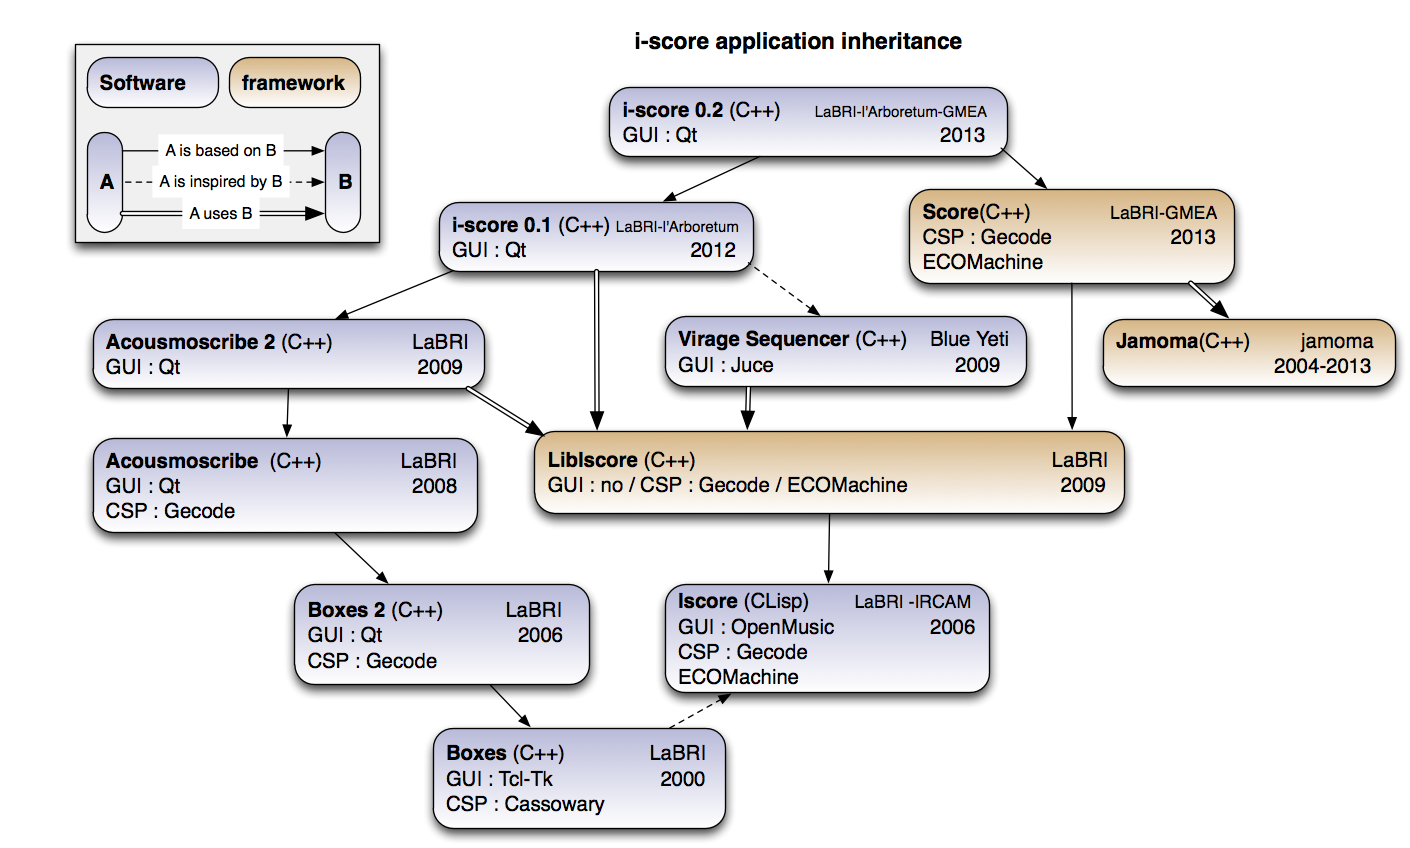
\includegraphics[scale=0.4]{images/iscoreHeritage.png}
	\caption{Les racines du logiciel i-score}
	\label{figheritageIScore}
\end{figure}

Actuellement, il incarne à la fois l'outil permettant d'écrire les scénarios, et de les exécuter.

Deux versions d'i-score (captures d'écran en \cref{figIScore}) sont en développement parallèle : i-score 0.2, une version fonctionnelle mais qui n'inclut pas les travaux les plus récents du paradigme \ac{OSSIA}, et i-score 0.3, une version pour l'instant non-fonctionnelle, mais qui a pour vocation de représenter l'état actuel du développement théorique.

\begin{figure}[H]
	\centering
	\begin{subfigure}{.5\textwidth}
		\centering
		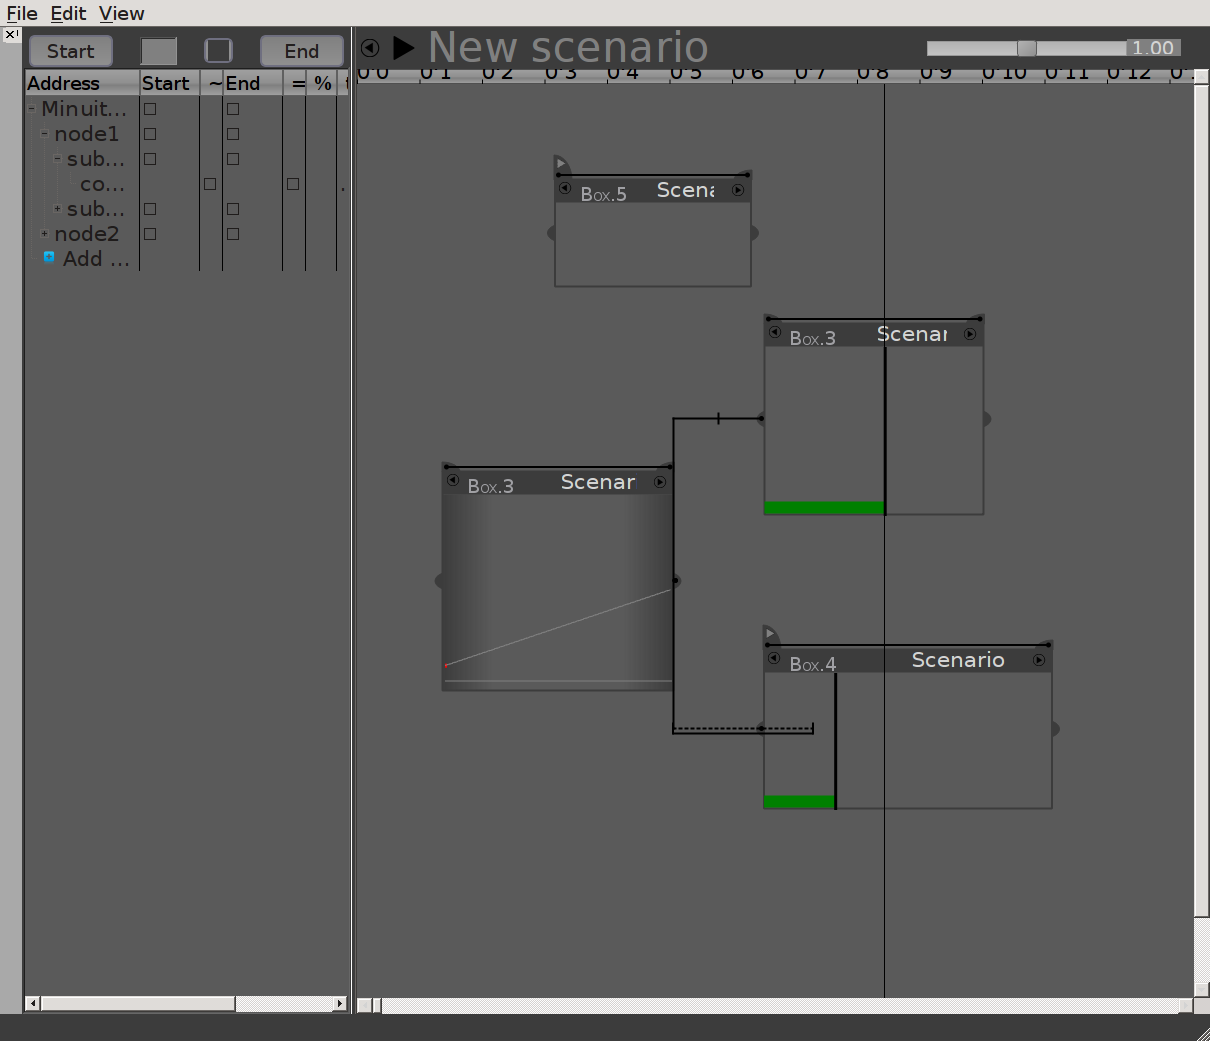
\includegraphics[scale=0.2]{images/iscore02.png}
		\caption{Version 0.2}
	\end{subfigure} 
	
	\vspace{1em}
	
	\begin{subfigure}{.5\textwidth}
		\centering
		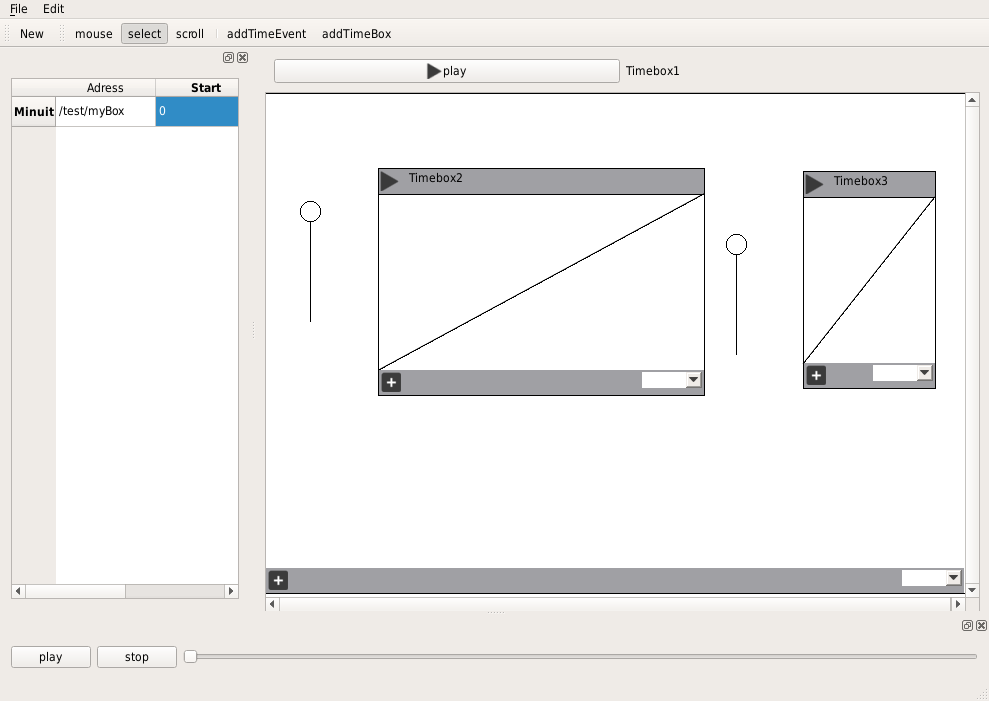
\includegraphics[scale=0.2]{images/iscore03.png}
		\caption{Version 0.3}
	\end{subfigure}
	
	\caption{Captures d'écran des deux version d'i-score.}
	\label{figIScore}
\end{figure}

\subsection{Score et API OSSIA}
\subsubsection{Score}
Score est la bibliothèque sous-jacente qui comporte la logique utilisée pour faire l'exécution d'i-score. Elle contient différents moteurs :

\begin{itemize}
	\item Un moteur d'exécution à base de réseaux de Petri.
	\item Un résolveur de \ac{CSP}, utilisé pour l'édition et plus spécifiquement le déplacement des boîtes.
\end{itemize}

Cette bibliothèque utilise le cadriciel \brand{Jamoma}.

\subsubsection{API}
La version 0.3 d'i-score se base sur une \ac{API}, qui offre toutes les possibilités de gestion de scénario directement au programmeur, de manière à ce que d'autres applications puissent être conçues par dessus. Par exemple, des acteurs du jeu vidéo sont intéressés par le fonctionnement offert par \ac{OSSIA} dans un environnement \brand{Unity}. 

\section{Organisation au cours du stage}
Cette partie précisera le déroulement de mon stage : compréhension du sujet, recherche, implémentation\dots

Pour rappel, le sujet précis du stage était : 
\begin{center}
	\noindent\fbox{\parbox{31em}{Répartition du séquenceur multimedia i-score sur plusieurs machines}}
\end{center}

L'énoncé complet du sujet est disponible en \cref{apx.SujetStage}.
\subsection{Attentes}
\label{sectionAttentes}
Les différents acteurs du projet ont tous eu des attentes différentes par rapport à mon stage.

Néanmoins, il est ressorti des réunions les points suivants : 
\begin{itemize}
	\item La répartition peut être faite au niveau des processus ou des scénarios.
	\item Il est nécessaire de pouvoir grouper facilement les parties sensées s'exécuter sur une même machine.
	\item Le backup doit être rendu possible.
	\item Le choix de synchroniser ou non est laissée au compositeur.
	\item Un des intérêts principaux est l'embarqué, que ce soit sur des micro-ordinateurs comme \brand{Raspberry Pi} et \brand{BeagleBoard}, ou bien sur des smartphones et tablettes tactiles.
	\item Le processus de composition doit pouvoir lui aussi être réparti (ou du moins accessible à plusieurs utilisateurs simultanément).
	\item Le formalisme doit être modifié pour prendre en compte la répartition.
	\item L'interface utilisateur doit être modifiée de manière à pouvoir cacher les parties qui s'exécutent à distance.
	\item Une interface utilisateur "chef d'orchestre" doit être présente et permettre de pouvoir tout voir et tout modifier.
\end{itemize}

Au niveau de la répartition, plus précisément, deux possibilités principales ont été vues comme désirables par les compositeurs : 
\begin{itemize}
	\item Le déplacement : le fait de déporter l'exécution d'un processus ou scénario sur une autre machine.
	\item La duplication : le fait de copier l'exécution d'un processus ou scénario sur une autre machine.
\end{itemize}

La duplication peut avoir une arité définie ou indéfinie, c'est à dire que le nombre de machines n'est pas forcément connu à l'avance.

Au niveau plus précis des processus, il a été envisagé de concevoir des cas particuliers permettant notamment de réaliser des opérations sur un groupe de signaux entrants. Par exemple, si onze machines sont lancées, dont une "maître" et dix exécutant un sous-scénario spécifique, on veut que les dix puissent agir chacune indépendamment sur un paramètre donné, et prendre comme résultat la moyenne, la somme, le minimum, le maximum, ou autre, de la valeur de ce paramètre sur les dix machines.

\subsubsection{Example dans le formalisme}
Un exemple, présenté en \cref{fig.RepartOSSIA}, a été conçu pour permettre de mettre en valeur les possibilités offertes.

Il est inspiré de l'exemple canonique du moine d'\ac{OSSIA}, présent en \cref{apx.OSSIAExemple}, et suit la même nomenclature.

\begin{figure}[h]
	\centering
	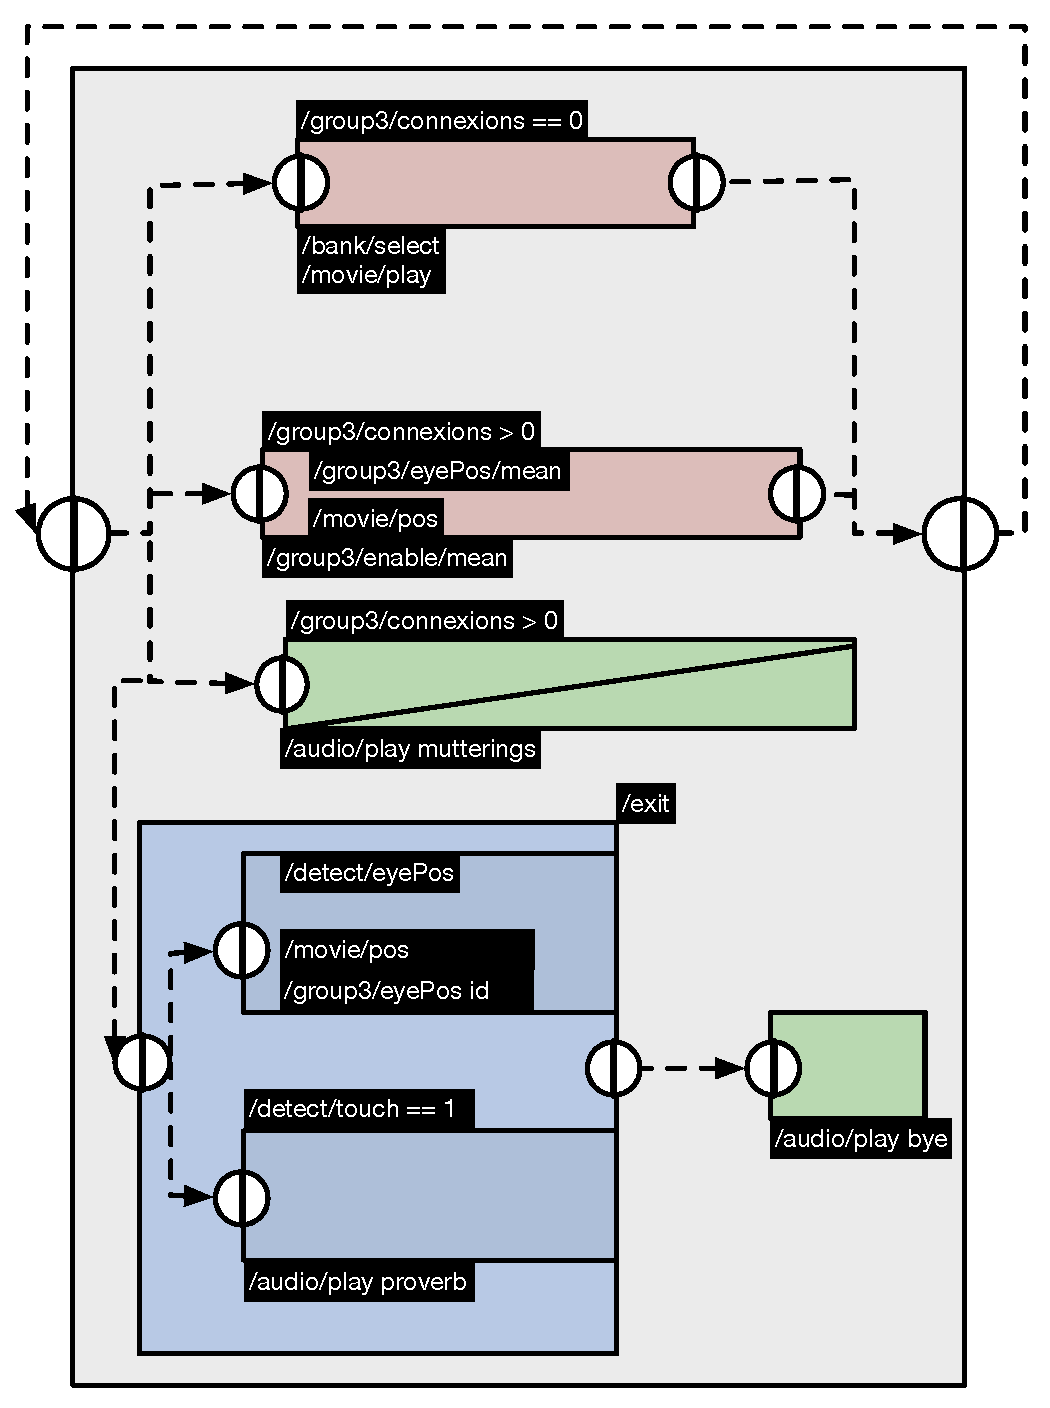
\includegraphics[scale=0.7]{images/ossiaDistri.pdf}
	\caption{Example de répartition dans le formalisme \brand{OSSIA}.}
	\label{fig.RepartOSSIA}
\end{figure}

Les couleurs représentent les groupes.
Il y a ici trois groupes : 

\begin{enumerate}
	\item Le premier groupe, \textcolor{BrickRed}{rouge}, sert à projeter de la vidéo sur un écran géant.
	\item Le second groupe, \textcolor{OliveGreen}{vert}, sert à lire des fichiers sons dans une salle.
	\item Le troisième groupe, \textcolor{SteelBlue}{bleu}, est exécuté sur un nombre quelconque d'appareils, comme des tablettes tactiles.  
\end{enumerate}

Le fonctionnement est le suivant : 
\begin{itemize}
	\item Quand personne n'est connecté, des vidéos quelconques sont jouées sur le vidéoprojecteur.
	\item Quand quelqu'un est connecté, il voit sur sa tablette un moine apparaître, qui suit le mouvement de ses yeux.
	\item Quand quelqu'un touche sa tablette, le moine de sa tablette récite un proverbe.
	\item Quand quelqu'un est connecté, un moine s'affiche sur l'écran géant. Le moine regarde dans la direction moyenne des moines présents sur les tablettes connectées au système. Des murmures sont aussi joués par le système de son, avec une augmentation continue et linéaire d'un paramètre (comme volume), puis son retour à zéro.
	\item Quand quelqu'un se déconnecte, un message d'au revoir est dit dans la salle.
\end{itemize}

Les dispositifs suivants sont nécessaires pour exécuter ce scénario : 
\begin{itemize}
	\item Une machine dédiée à l'audio reliée au système de son.
	\item Une machine dédiée à la vidéo reliée au vidéoprojecteur.
	\item Un ensemble de tablettes ou téléphones tactiles avec une caméra en face avant, un logiciel de vidéo, et logiciel d'eye-tracking.
\end{itemize}

Il n'y a pas besoin de machine spécifiquement maîtresse : une des deux machines audio ou vidéo peut en faire office.
Néanmoins, une telle machine peut être rajoutée.
\subsection{Problèmes posés par la répartition}
Un des problèmes majeurs ici est le besoin de synchronisation avec une horloge physique. En effet, les relations entre débuts et fins d'évènements sont données sous forme de millisecondes les séparant, les réseaux étant temporels. Ainsi, les mécanismes d'horloges vectorielles et logiques ne sont pas directement applicables.

Le deuxième problème est qu'il n'est pas réellement question de répartition au sens couramment entendu dans le domaine de l'informatique répartie. En effet, ici, les processus correspondent à des besoins physiquement présents sur des machines et qui ne peuvent pas être déplacés sur d'autres machines. Par exemple, une machine peut avoir une sortie vidéo, et une autre machine une carte son : cela conditionne pour le compositeur l'endroit ou s'exécute un processus, selon qu'il soit relatif à l'image ou au son.

Idéalement, il serait possible de faire une différenciation automatique, néanmoins, deux aspects s'y opposent : 
\begin{itemize}
	\item Le compositeur désire avoir le choix pour la répartition.
	\item Score ne communique qu'avec des messages \ac{OSC}. Un message \ac{OSC} a le format suivant : 
	\begin{verbatim} /adresse/où/écrire argument1 argument2 ... \end{verbatim}.
	
	Les adresses sont laissées à la discrétion des logiciels avec lesquels Score communique, car non standardisées. Il n'est donc pas possible de savoir quel type d'information est communiqué. 
\end{itemize}
Un troisième point, limitant, à tenir en compte, est celui de la gestion de l'interactivité. Dans ce cas, l'impact de la latence due au réseau physique est inévitable, si par exemple un artiste décide d'activer une fonction qui est sensée s'exécuter sur une autre machine.


\subsection{Définition du travail à réaliser}
Étant donné la nature duale du stage, mon travail a été séparé en deux parties qui se sont précisées au fil des réunions avec mes encadrants.

\subsubsection{Recherche théorique sur les réseaux de Petri}
Il est apparu assez clairement que la majorité de mon travail théorique porterait sur les réseaux de Petri, car l'intérêt majeur est d'avoir une exécution répartie des scénarios.

J'ai donc essayé de réaliser un existant à jour sur ce sujet, ainsi que sur celui des dernières avancées en répartition et en synchronisation de machines et d'horloges.
Néanmoins, malgré des rencontres avec plusieurs enseignants, je n'ai pas trouvé d'existant portant spécifiquement sur l'exécution des réseaux de Petri dans un cas réparti.
Cette phase est détaillée au \cref{chapterStateOfTheArt}.

Par la suite, j'ai essayé de concevoir des méthodes théoriques pouvant répondre au problème.
J'ai ensuite choisi celle qui a semblé la plus pertinente en les comparant, et ai essayé de prouver sa correction, ainsi que de proposer des améliorations.
Ce travail est présenté dans le \cref{chapterApports}.

\subsubsection{Travail de conception}
La conception a été divisée en trois parties : 
\begin{itemize}
	\item Choix des technologies à utiliser et de la position ou mon travail doit se situer.
	\item Conception d'un logiciel de test de répartition de réseaux de Petri.
	\item Intégration des idées présentées en \cref{sectionAttentes} dans i-score.
\end{itemize}

Elle a été suivie d'une phase d'implémentation.

Les détails se trouvent au \cref{chapterImpl}.
\subsection{Organisation temporelle}
(TODO mettre diagramme de Gantt)
\chapter{État de l'art}
\label{chapterStateOfTheArt}
L'état de l'art des domaines relatifs à ce stage s'intéressera à trois aspects : 
\begin{itemize}
	\item Les avancées en réseaux de Petri, qui sont au cœur du modèle.
	\item Les avancées en terme de répartition, et de synchronisation en temps entre machines.
	\item L'état actuel du projet \ac{OSSIA}. 
\end{itemize}

Quand ils ne sont pas semblables au français, les noms anglais des termes scientifiques employés seront marqués en \textit{italique}.

\section{Réseaux de Petri}
Les réseaux de Petri\cite{petri1962kommunikation} sont au cœur du formalisme utilisé ici. Néanmoins, une différence majeure entre leur utilisation dans le projet \ac{OSSIA} avec d'autres utilisations plus courante est que pour \ac{OSSIA}, les réseaux ne servent pas à faire de l'analyse statique mais sont au cœur du moteur d'exécution du programme. C'est-à-dire que la théorie des scénarios a été développée de manière à pouvoir être exprimée en terme de réseaux de Petri, et que ces réseaux de Petri sont ensuite exécutés avec un algorithme relativement simple, qui sera détaillé plus tard dans ce document.

La conférence principale sur le thème des réseaux de Petri est l'\textit{International Conference on Application and Theory of Petri Nets and Concurrency}, qui présente cette année sa 35\ieme édition.

\subsection{Familles de réseaux de Petri}
À l'origine, les réseaux portaient le nom de réseaux places-transitions. La définition la plus simple est celle d'un graphe orienté biparti, dont les deux parties sont les places, et les transitions.

Les places contiennent des jetons; quand les places antécédentes à une transition possèdent toutes au moins un jeton, celle-ci est dite \textit{sensibilisée}. Elle peut alors s'exécuter (on dit qu'elle est \textit{tirée}) en enlevant un jeton à chaque place la précédant et en rajoutant un jeton à chaque place la suivant.

Plusieurs cours et livres récents présentent les généralités des réseaux de Petri \citep[voir][]{david2010discrete, diaz2013petri}, avec les notations et vocabulaires contemporains.

Néanmoins, étant un formalisme facilement extensible, plusieurs modifications des réseaux de Petri ont prouvé leur intérêt; elles seront vues plus en détail dans les prochains paragraphes.
\subsubsection{Réseaux hiérarchiques}
L'idée de base des réseaux hiérarchiques consiste à avoir des sous-réseaux qui s'exécutent lorsqu'un jeton arrive dans une place.

Une extension aux transitions existe, en utilisant la notion de blocs de construction\cite{fehling1993concept}.

Actuellement, l'essentiel de la recherche dans ce domaine consiste en la recherche de formalisations pouvant généraliser les différents concepts de modularité, comme par exemple \brand{LLAMAS} (Language for Advanced Modular Algebraic Nets)\cite{colom2013application}.

Les réseaux hiérarchiques sont principalement utilisés pour modéliser des systèmes complexes du monde réel, dans des cas industriels par exemple.

\subsubsection{Réseaux colorés}
Les réseaux colorés\cite{zervos1977colored,jensen1987coloured} ont été une des premières extensions des réseaux de Petri. L'idée principale est de permettre aux jetons d'être porteurs de donnée, à l'aide des couleurs. 

Les transitions peuvent créer des jetons de couleur, et les arcs possèdent des fonctions d'arc laissant passer les couleurs choisies.

La notion de hiérarchie a été étendue aux réseaux colorés de plusieurs manières différentes \cite{rozenberg1991advances}, qui sont à choisir en fonction des cas d'utilisation.

Une généralisation des réseaux colorés porte le nom de réseaux de haut niveau (\textit{high-level Petri nets}) \cite{jensen1983high}. Elle remplace la notion de couleur par celle de type, plus extensible.
Il est possible de convertir des machines à état \brand{UML} en réseaux de Petri de haut niveau en utilisant un algorithme génétique \cite{alhroob2014transforming}.

\subsubsection{Réseaux liés au temps}
Il existe plusieurs manières d'introduire la notion de temps dans les réseaux de Petri.
\begin{itemize}
\item La première méthode a été celle des réseaux temporisés (\textit{timed Petri net}) : les places ou transitions portent les durées des actions qu'elles simulent. C'est le cas d'i-score.

\item Peu après a été établi le formalisme des réseaux temporels (\textit{time Petri net}) : les éléments du réseau (place ou transition) peuvent avoir une date minimale et maximale d'exécution.
Une extension récente \cite{klai2013temporal} au dessus des réseaux temporels  présente un moyen d'encoder le temps minimal et maximal écoulé à chaque instant, ainsi que les avantages que cela peut avoir.

\item Enfin, le modèle relatif au temps le plus récent utilise les opérateurs de logique temporelle \cite{logic2002temporal,suzuki1989temporal}. L'avantage par rapport aux modèles temporels et temporisés est une meilleure représentation des propriétés de vivacité (\textit{liveness}).
\end{itemize}
\paragraph{Réseaux stochastiques}
Les réseaux de Petri stochastiques \cite{bause1996stochastic} sont d'une certaine manière reliés au temps.

Dans ce type de réseau, les transitions franchissables sont activées après un délai déterminé par une variable aléatoire.
 
\subsubsection{Réseaux flous}
Les réseaux de Petri flous (\textit{fuzzy Petri nets}) \cite{pedrycz1994generalized} sont une classe de réseau de Petri inspirés des réseaux neuronaux. Leur utilité principale est comme pour les réseaux neuronaux l'apprentissage informatique.

Une approche récente utilise les réseaux de Petri flous pour modéliser des systèmes à connaissance floue\cite{wang2014dynamic}, et plus généralement les systèmes de modélisation de la connaissance, en prenant en compte la notion d'incertitude.

\subsection{Standardisation}
Il est assez apparent au vu de la section précédente que les variations autour du formalisme de base sont assez ample, et que beaucoup d'extensions sont possibles.

Un effort de standardisation est mené depuis le début des années 2000 pour avoir un format d'échange commun à différents outils, avec le langage \ac{PNML}.

Cet effort a abouti en 2008 et 2011 avec la standardisation dans la norme ISO/IEC 15909-2.

Le langage est basé sur du \brand{XML}, avec une attention importante à la modularité. Il a été conçu à l'aide de \glspl{metamodel} \brand{UML}.

Un état de l'art\cite{hillah2010standardisation} a été dressé par les auteurs du langage en 2010.

L'accent actuel est mis sur la gestion de la modularité, avec l'implémentation des concepts de hiérarchie, ou d'encapsulation. Ce travail est réalisé dans \brand{Modular PNML}. Un méta-modèle pour représenter les réseaux de Petri modulaires est en cours d'étude\cite{marechal2012modular}.

\subsection{Outils développés pour l'analyse des réseaux de Petri}
En sus de la théorie bâtie depuis bientôt un demi-siècle, les réseaux de Petri sont aussi très utilisé en pratique, pour réaliser des simulations de systèmes à complexité variable.

(TODO mettre captures d'écran ?)

\subparagraph{ePNK} est une plateforme logicielle travaillant en format \ac{PNML}. Elle est bâtie autour de la notion d'extensibilité, en permettant aux autres développeurs d'insérer facilement leurs propres formalismes de réseaux de Petri avec une architecture en plug-in.

À la base prévue pour l'édition, elle est aussi désormais capable de simuler l'exécution de réseaux de Petri  \cite{kindler2013simulator}.

\subparagraph{PetriNet API} \cite{lohmann2009petri} est une interface de programmation en \brand{C++} offrant aux développeurs des structures de données simples (place, transition, réseau de Petri) permettant de bâtir leurs propres outils par dessus.

Un des avantages est l'import de données au format \ac{PNML} et l'export au format \brand{DOT} de \gls{graphviz}, à des fins de visualisation.

\subparagraph{CPN Tools} (\textit{Colored Petri Net Tools}) permet comme \brand{ePNK} d'éditer, simuler, et analyser des réseaux de Petri colorés \cite{jensen2007coloured}.

Il est notamment utilisé dans le projet \ac{OSSIA} à des fins de validation.

\subparagraph{PNlib} \cite{pross2014object} est un outil de simulation orienté objet visant le cas particulier des processus biologiques.

La bibliothèque a été réalisé en \gls{modelica} et s'y intègre facilement.

\subparagraph{Snoopy} \cite{heiner2012snoopy} est un autre cadre logiciel à vocation unificatrice, permettant aussi l'utilisation de la couleur. Il supporte la hiérarchie.

Des outils d'analyse dynamique sont intégrés au logiciel.

Il a été appliqué aux réseaux biomoléculaires \cite{rohr2010snoopy}.

Une des particularités du logiciel est d'avoir plusieurs vues pour le même modèle, et d'aleterner facilement entre ces vues. Par exemple, il est possible d'avoir un modèle stochastique et un modèle continu pour le même réseau, qui partagent certaines propriétés.

\subsection{Applications récentes}
Il serait très dur d'établir un inventaire complet des utilisations des réseaux de Petri : comme pour les automates, les machines de Turing, ou encore le lambda-calcul, c'est un outil avec une très forte puissance d'expression, qui peut donc être utilisé dans une variété d'environnements différents, à des fins de modélisation.

Par exemple, à l'origine, C. A. Petri avait conçu les réseaux qui portent aujourd'hui son nom afin de modéliser des réactions chimiques. Ils sont maintenant très utilisés dans les modélisations de comportements biologiques \cite{koch2014petri}.

\subsubsection{Parallélisme}
Une des applications les plus courantes des réseaux de Petri est de simuler des systèmes répartis.

Un domaine annexe est celui de la parallélisation. Récemment, des progrès ont été fait dans la gestion de l'ordonnancement dans le cas d'applications s'exécutant en parallèle\cite{chen2014research}. Notamment, le système est modélisé à l'aide d'un réseau de Petri, et un algorithme génétique est utilisé pour y rechercher un chemin permettant un temps d'exécution minimal. 

\subsubsection{Application aux interfaces homme-système}
Les réseaux de Petri peuvent servir à modéliser toutes sortes de systèmes se basant sur une succession d'évènements.
 
Ils ont par exemple été utilisés pour la modélisation des interactions homme-système\cite{campos2014elementary}, avec différentes catégories d'évènements, comme le dépassement d'un seuil ou l'émission d'un signal, ce qui permet par la suite d'effectuer une analyse statique qui pourrait montrer des failles dans la conception du dit système.

\subsubsection{Application à des modèles cyber-physiques}
La \gls{cyberphysique} peut tirer un certain bénéfice des réseaux de Petri pour la simulation de son bon fonctionnement. En effet, elle consiste en différents éléments répartis et communiquants.

Des réseaux de Petri spatio-temporels ont été introduits\cite{zhang2014modeling} pour gérer les aspects de déplacements physique au cours du temps dans ce cas.

\section{Répartition}
La répartition (\textit{distribution}) est un second point important de ce stage. C'est un domaine qui est souvent très proche de la technique : le besoin d'utiliser des algorithmes répartis provient souvent de contraintes matérielles ou temporelles.

\subsection{Ouvrages de référence}
Plusieurs livres sont dédiés à des présentations générales du sujet, celui-ci étant étudié depuis plusieurs décénnies.

Au niveau des algorithmes, le livre de Nancy Lynch \cite{lynch1996distributed} présente les cas et problèmes les plus courants, en séparant les méthodes synchrones et asynchrones. 

Un autre ouvrage \cite{attiya2004distributed} met plus l'accent sur la simulation d'algorithmes distribués.

\subsection{Vérification}
La vérification des algorithmes distribués est une branche majeure qui nécessite des outils particuliers par rapport aux méthodes formelles usuelles, comme la \gls{logiquedehoare} telle qu'elle fut définie à l'origine par exemple.

Les outils de base sont la sécurité (\textit{safety} et la vivacité \textit{liveness}), telles qu'énoncées par Leslie Lamport \cite{lamport1977proving}.

De nombreux articles plus ou moins récents sur ce sujet sont référencés par un laboratoire de l'université de l'Illinois \cite{formaldistributed}.

Un des aspects particulièrement important dans le cas d'algorithme distribué est celui de la tolérance aux pannes. Par exemple, comment faire si un câble est débranché ? Et, plus précisément ici, comment vérifier qu'un algorithme donné sera tolérant aux pannes possibles ? 

Un exemple est donné \cite{mcmillan2014verification} pour le cas des algorithmes de consensus, qui introduit une logique de premier ordre particulière (nommée \textit{Consensus verification logic}).

Une autre approche utilisée est celle des algorithmes de transmission de messages \cite{jezequel2014message}, qui a été appliquée à la vérification de certains protocoles distribués, comme par exemple un protocole de \gls{mutex}.

\subsection{Développement}
Cette partie traitera des publications récentes ayant trait à l'implémentation des algorithmes de répartition.

Un ouvrage récent \cite{varela2013programming} fait le lien entre la théorie et la pratique, en présentant les méthodes les plus récentes pour écrire certains algorithmes. Un accent est mis sur la manière dont différents langages de programmation vont permettre plus ou moins simplement de réaliser différents paradigmes. Il tient aussi compte des avancées sur le \gls{calculambiant}, le \gls{picalcul}, et le \gls{joincalcul}.

\subsubsection{Modèles au fait des données (\textit{data-aware})}
Un algorithme opère toujours sur des données, néanmoins les opérations relatives à ces dernières (déplacement, envoi...) sont souvent considérées comme secondaires et comme quelque chose sur lesquelles l'auteur de l'algorithme distribué n'a pas de pouvoir.

Néanmoins, avec l'avènement du \gls{bigdata}, il est nécessaire de mieux prendre en compte cet aspect, parfois au niveau du système d'exploitation, ou encore des protocoles de routage utilisés \cite{baehni2004dependable} car les effets de bord deviennent trop volumineux.

Ainsi, des nouveaux paradigmes d'ordonnancement ont été proposés \cite{yildirim2012data, kosar2009paradigm}, ainsi que des méthodes pour optimiser le transfert de ces données.

\subsubsection{Routage}
Le routage est une problématique centrale des systèmes répartis, l'idéal étant de minimiser son temps.

Une méthode a été récemment proposée pour réduire ce temps en cas de forte charge sur les lignes, mais uniquement dans des cas de réseaux statiques \cite{jeon2014fully}.

% % % % Modularity in the design of robust distributed algorithms

De plus, il est intéressant de noter que des problèmes de routage comme la gestions des congestions peuvent s'appliquer à d'autres types de réseaux que les réseaux informatiques. Par exemple, des algorithmes ont été développés pour gérer en temps réel les problèmes des feux de circulation \cite{aoxue2014distributed}, en s'inspirant du concept de \gls{mutex} et en utilisant des capteurs embarqués sur chaque véhicule.

\subsubsection{Réseaux sans-fil}
Les réseaux sans-fil sont désormais omniprésents, et offrent de nouvelles opportunités d'optimisation qui leur sont propres.

Par exemple, il a été montré dans \cite{hosseinabadi2014exploiting} que les paquets entendus par un client mais qui ne lui étaient pas directement destinés (\textit{overheard packets}) pouvaient être utilisés pour améliorer la performance du réseau (et notamment les temps d'attentes dûs aux collisions), à l'aide d'algorithmes spécifiques.

Un outil, \brand{FlockLab} \cite{lim2013flocklab} a été conçu spécifiquement pour la vérification et l'analyse de réseaux sans-fil embarqués. Il permet le débogage, et l'étude des timings à une précision proche de la microseconde en utilisant les protocoles généralement utilisés sur l'embarqué, comme \ac{GPIO}.  

\section{Synchronisation}
Les problèmes de synchronisation sont généralement vus comme une sous-partie des problèmes inhérents aux systèmes embarqués. Néanmoins, dans ce sujet, c'est une des partie les plus importantes et pertinentes, d'où l'accent qui y est apporté.

La synchronisation implique toujours un concept d'horloges. Deux branches sont étudiées : les horloges logiques, qui servent à ordonner les éléments entre eux, et les horloges physiques, qui servent de référence absolue.

\subsection{Synchronisation logique}
\subsubsection{Origines : les horloges de Lamport}
Le premier système d'horloge logique est celui conçu par Leslie Lamport, récipient du prestigieux \textit{Turing Award 2013}.

Il a notamment conçu les horloges et horodatages qui portent son nom, et qui expriment la notion de "arrivé-avant".
\subsubsection{Horloges vectorielles}
Les horloges vectorielles (\textit{vector clocks}) sont une amélioration au dessus du concept des horloges de Lamport.

Néanmoins, plutôt que de ne faire garder que leur état logique aux nœuds, on leur fait garder l'état de tous les nœuds dont ils ont reçu des messages dans un vecteur. Lorsqu'un nœud envoie un message à un autre, ce dernier se met à jour avec les horodatages maximaux contenus dans le vecteur qui est envoyé.

Le problème des horloges vectorielles est la croissance de la taille du vecteur dans un système contenant beaucoup de nœuds.

\paragraph{Horloges plausibles}
Plausible clocks: constant size logical clocks for distributed systems

\subsection{Synchronisation physique}
Comme i-score est un logiciel permettant de manipuler le temps, il nécessite de travailler avec une horloge physique. Le problème principal des systèmes distribués se basant sur une horloge est de s'assurer que tous les nœuds ont la même heure.

\subsubsection{Algorithmes couramment utilisés}
En pratique, il existe deux méthodes couramment utilisées pour garantir une synchronisation des horloges entre machines.

\subparagraph{NTP} (\textit{Network Time Protocol}) est la méthode couramment utilisée sur Internet pour synchroniser l'heure des machines.

Elle emploie une structure en arbres avec plusieurs niveaux, chacun communiquant uniquement avec ses niveaux supérieurs et inférieurs.

Elle permet une synchronisation de l'ordre de (TODO)
\subparagraph{PTP} (\textit{Precision Time Protocol}) est une méthode qui a été développée après \brand{NTP}, et qui est optimisée pour les réseaux locaux requérant une plus grande précision que celle que peut offrir \brand{PTP}.

Elle permet une synchronisation de l'ordre de (TODO)

\ac{PTP}
Cf. articles sur précision sur Android : 
A Measurement of Time synchronization on Mobile Devices.

Comparer avec NTP + implémentation existantes.

\subsubsection{Travaux plus récents}
(TODO mieux catégoriser)
Distributed synchronization under uncertainty: A fuzzy approach

Fine-grained network time synchronization using reference broadcasts

Subscription-Notification mechanisms for synchronization of distributed states

One Clock to Rule Them All: A Primitive for Distributed Wireless Protocols at the Physical Layer

Distributed network synchronization: the internet and electric power grids

Riccati Design for Synchronization of Discrete-Time Systems (bof)

Riccati Design for Synchronization of Continuous-Time Systems

Time Synchronization for High Latency Acoustic Networks


\subsection{Estimation de la latence}
\label{section:latence}
Network latency estimation % http://www.google.com/patents/US8254264B1

King: estimating latency between arbitrary internet end hosts

Method and system for peer-to-peer network latency measurement % http://www.google.com/patents/US6012096


\section{Projet OSSIA}
Le projet \ac{OSSIA}

(Présentation travaux Allombert, Toro, Arias, etc.)

Modelling Data Processing for Interactive Scores Using Coloured Petri Nets


\subsection{Les réseaux de Petri dans OSSIA}
\subsection{Scénarios interactifs}
\subsection{Temps souple}
\subsection{Exemple dans le formalisme OSSIA}


\chapter{Apports au problème}
\section{Introduction}
Le but de cette partie est de fournir une sémantique  personnalisée pour la distribution de l'exécution d'un réseau de Petri sur un réseau informatique, en prenant en compte les délais dûs à la répartition physique des machines et les contraintes issues du projet \ac{OSSIA}.

\subsection{Rappel du formalisme}
Le formalisme de base utilisé est celui des réseaux de Petri t-temporisés, disposant d'un couple place $\rightarrow$ transition initiale et transition $\rightarrow$ place finale, avec pour restriction le fait qu'une place ne puisse posséder qu'une entrée et qu'une sortie, et ce pour éviter les problèmes de conflits et confusions. L'utilisation de la couleur est possible.

Les réseaux de Petri utilisés ici sont connexes : la seule place n'étant pas en sortie de transition est la place initiale, et la seule place n'étant pas en entrée de transition est la place finale.

\subsubsection{Algorithme d'exécution de base}
(TODO rédiger avec algorithm2e)
Un jeton est placé dans la place initiale, le temps est initialisé à 0. Une horloge est initialisée.

Pour chaque transition, si elle est sensibilisée, et que la somme des durées entre elle et la place initiale est écoulée, alors elle est franchie.

Quand tous les jetons ont franchi la transition menant à la place finale, l'algorithme termine.

\paragraph{Note} Il est possible que l'algorithme ne termine pas : en effet, on pourrait vouloir un scénario en boucle infinie, pour une installation artistique par exemple.

\subsection{Démarche suivie}
La première étape de mon travail a été de rechercher l'existant proche du cas présent. Néanmoins, malgré diverses rencontres avec des professeurs spécialisés dans le domaine des automates et des réseaux, et une recherche bibliographique sur ce sujet, aucun autre cas de moteur d'exécution de réseau de Petri n'a été trouvé.

Ainsi, ma recherche s'est plutôt portée sur les moyens de répartir des algorithmes à la base prévus pour une utilisation sur une seule machine. 

L'idée principale a été de lancer les exécutions des sous-scénarios répartis sur d'autres machines en avance.

Cela engendre deux problèmes : 
\begin{itemize}
\item Comment estimer le retard entre deux machines ?
\item Comment modifier les réseaux de Petri de manière à ce qu'ils prennent en compte le départ en avance qui en découle ?
\end{itemize}

C'est surtout le second qui est au cœur de cette partie, le premier étant couvert de manière extensive par la littérature scientifique.

Trois idées différentes pour parvenir à ce but sont présentées : deux qui se basent sur la modification de la topologie du réseau, et une qui se base sur la modification de la sémantique du réseau.

De plus, la notion de segment est introduite, qui est une légère abstraction permettant de représenter simplement les processus dans les réseaux de Petri.

\section{Définitions}
Un des problèmes de vocabulaire principal dans ce document est que nous faisons référence à deux types de réseaux tout à fait distincts : les réseaux de Petri, et les réseaux informatiques présents dans le monde physique.

Pour pallier ce problème, nous utiliserons de préférence l'idée de graphe quand il s'agit de réseau informatique, et l'idée de réseau quand il s'agit de réseau de Petri.

\subsection{Définitions relatives aux réseaux physiques}
\begin{mydef}
Un réseau informatique est représenté par un graphe orienté $G$ dont les nœuds représentent les machines, et les arêtes les liens entre ces machines. 

Les arêtes sont étiquetées par un temps $\delta$, signifiant le temps de transmission d'un message entre les deux nœuds attenants à l'arête.
\end{mydef}
$\delta$ sera considéré fixe. Néanmoins, dans un scénario réel, il serait envisageable (et recommandé) de mesurer et corriger $\delta$ régulièrement en raison de la latence entre les nœuds qui peut varier, notamment à l'aide des méthodes présentées en partie \ref{section:latence}.

(TODO faire thm propre pour notation) \\
Notation : soient $N_1$ et $N_2$ deux nœuds du graphe. On note $\delta_{N_1 \rightarrow N_2}$ le temps de transmission entre $N_1$ et $N_2$. 

Bien que dans de nombreux cas, $\delta_{N_1 \rightarrow N_2} \simeq \delta_{N_2 \rightarrow N_1}$, nous ne ferons pas cette supposition ici. En revanche, nous considérerons toujours des liens en duplex.

Les nœuds de $G$ peuvent contenir des places et des transitions. Si un nœud contient une transition, on dit qu'il l'\textit{exécute}.

\subsection{Définitions relatives aux réseaux de Petri}
\begin{mydef}
Un segment est composé d'une transition, de ses $N$ places d'entrées, et de ses $M$ places de sortie, avec $N \geq 1, M \geq 1$.
\end{mydef}

On notera que mis à part les segments initiaux et finaux, tous les segments partagent au moins une place avec un autre segment.

L'approche utilisée dans les schémas de ce document est de représenter un segment par ses places d'entrée et sa transition.

\begin{mynot}
On note $\entree(s)$ l'ensemble des places d'entrée de $s$, $\sortie(s)$ l'ensemble des places de sortie de $s$.
\end{mynot}

\begin{mynot}
On note $\pre(s)$ l'ensemble des segments précédant le segment $s$, $\post(s)$ l'ensemble des segments suivant $s$.
\end{mynot}

\begin{mynot}
On note $\shared(s_1, s_2)$ les places en sortie de $s_1$ et en entrée de $s_2$.
\end{mynot}

\section{Méthodes par modification de la topologie}
\chaptermark{Premières méthodes}
Ces formalisations se font par modification de la topologie du réseau de Petri. C'est-à-dire que des places, arcs, et transitions vont être rajoutées au réseau pour encoder la notion de départ en avance.

\subsection{Définitions}
\subsubsection{Définition des opérations de transformation de base}
Deux niveaux d'opération sont décrits dans ce document.

Ici, on décrit les opérations atomiques pouvant être exécutées sur les segments, qui ne tiennent pas compte de la répartition. 

Par la suite, chaque méthode comportera ses propres opérations, qui serviront spécifiquement à appliquer la répartition. 

Toutes ces opérations seront écrites en police informatique : \texttt{maFonction(x)}.

Il convient de noter que les opérations appliquant la répartition sont réversibles. Ainsi, il est toujours possible d'appliquer les opérations atomiques sans avoir besoin de tenir compte de la répartition : il suffit d'inverser ces dernières, d'appliquer les opérations atomiques, puis de ré-appliquer les opérations de répartition effectuées, si possible (un cas impossible serait celui ou on voudrait supprimer un segment qui était réparti).

\paragraph{Création}
On considère la fonction \texttt{crée(d, nPlacesEntrée, nPlacesSortie)}. Elle permet de créer un segment, de durée \texttt{d} et avec un nombre explicite de places d'entrée et de sortie.

\begin{itemize}
\item \texttt{d} peut être une durée variable.
\item \texttt{nPlacesEntrée} $ \geq 1 $ et \texttt{nPlacesSortie} $ \geq 1 $.
\end{itemize}
\paragraph{Lien}
Le lien crée un arc entre deux segments.

On définit : \texttt{lie(sOrigine, pDestination)} qui crée un arc entre la transition du segment \texttt{sOrigine}, et la place \texttt{pDestination}.

De même, \texttt{délie(sOrigine, pDestination)} supprime un arc.

\paragraph{Suppression}
(TODO processus sur place partagée?)
\texttt{suppr(s)} supprime le segment, ainsi que les arcs en entrée et en sortie.

Si un segment ne se retrouve plus relié à rien suite à cette opération, une place d'entrée lui est rajoutée, qui est reliée en sortie de la transition initiale.

\subsubsection{Définition de segments particuliers}
(TODO cela aurait-il sa place dans la partie plus générale ? Moins utilisé dans formalisation par couleur...)

Ces segments relient les notions de graphe de machines et de réseau de Petri.
\begin{mydef}
Une transition non-distribuée, notée nd-transition, correspond à une transition dont aucune des places d'entrée ou de sortie ne sont situées sur un autre nœud du graphe.
\end{mydef}

\begin{mydef}
Une transition distribuée, notée d-transition, correspond à une transition dont une des places d'entrée ou de sortie est située sur un autre nœud du graphe.
\end{mydef}

\begin{mydef}
Un d-segment (resp. nd-segment) est un segment bâti autour d'une d-transition (resp. nd-transition).
\end{mydef}

\begin{mydef}
Deux segments sont dits consécutifs s'ils partagent au moins une place. Cela implique qu'au moins une place de sortie de l'un soit une place d'entrée de l'autre.
\end{mydef}

Un réseau de Petri distribué contient des d-segments et des nd-segments consécutifs, ainsi qu'une place initiale et une place finale.

Des processus existent de plus au-dessus de segments, qui sont signifiés par un changement d'état d'un paramètre entre deux places. Il est donc important d'assurer que la durée de ces processus ne change pas lors de la distribution. (TODO déplacer dans pbq)

\subsection{Première tentative de formalisation}
\subsubsection{Opérations définies sur segment}
On considère que dans l'état initial du système, tous les segments sont situés sur le même nœud.

\paragraph{Déplacement}
L'opération de déplacement consiste à déporter l'exécution d'un nd-segment d'un nœud vers un autre, en transformant le réseau pour s'accommoder des délais.

\subparagraph{Processus} ~ \\

On note $s$ le segment à déplacer.
Pour tout segment $p \in \pre(s)$ : 

\begin{enumerate}
\item Soit $t_p$ la durée de la transition de $p$. On change cette durée en $t_p - \delta$.
\item On rajoute une place en sortie de $p$ ainsi qu'une transition $T$ de durée $\delta$ à la suite de cette place. 

Pour tout segment $o$ appartenant à $\post(p)$ à l'exception de $s$, on supprime les arcs entre $o$ et $p$, puis on crée des arcs allant de $T$ aux places d'entrée de $o$.

On duplique de plus toute place appartenant à $\shared(p, s)$, en sortie de $T$, de manière à garder l'ancienne position de $s$ en mémoire pour annuler le déplacement si nécessaire.

On notes cet ensemble de places dupliquées $\memory(s, p)$ (la mémoire des places d'origine lors du déplacement de $s$ par rapport à $p$).
 
\item On déplace l'information de fin de processus potentiellement contenue sur les places de $\shared(p, s)$ vers les places  $\memory(s, p)$. Cela permet d'avoir les évènements de fin de processus attenants à $p$ exécutés sur le même nœud que $p$.
\end{enumerate}

Puis, on applique la même opération entre $s$ et les segments appartenant à $\post(s)$, pour avoir une compensation de délai par rapport aux nœuds des segments suivant $s$.

Un exemple graphique est présenté en figure \ref{fig:deplacementMethode1}.

\begin{figure}[h!]
\centering
On déplace s sur un nœud $N_d$ : 

\begin{tikzpicture}[node distance=1.3cm,>=stealth,bend angle=45,auto]

  \tikzstyle{segment}=[]
  \tikzstyle{place}=[circle,thick,draw=blue!75,fill=blue!20,minimum size=6mm]
  \tikzstyle{red place}=[place,draw=red!75,fill=red!20]
  \tikzstyle{transition}=[rectangle,thick,draw=black!75,
  			  fill=black!20,minimum size=4mm]
  			  
  \tikzstyle{black box}=[draw=black, fill=black!30, draw opacity=0.7, fill opacity=0.2, thick, dashed, inner sep=0.5cm]


  \begin{scope}
    \node [transition] (Tk) [label=$t_p$] {};
	\node [segment] (Pk) [left of=Tk] {$\pre(p)$};
	\node [segment] (S) [right of=Tk] {$s$};
	\node [segment] (Sk) [below of=S] {$\post(p) \setminus s$};
			
  	\path
  		(Pk) edge[post] node {} (Tk)
  		(Tk) edge[post] node {} (S)
  			 edge[post] node {} (Sk);
  
   \begin{pgfonlayer}{background}
    \node [black box, fit=(Tk) (Pk) (S) (Sk)] (Box1) {};
    \node[above right] at (Box1.south west) {Nœud $N$};
   \end{pgfonlayer}
  \end{scope}
  
  
\end{tikzpicture}

\vspace{1em}
Devient
\vspace{1em}

\begin{tikzpicture}[node distance=1.3cm,>=stealth,bend angle=45,auto]
 
   \tikzstyle{segment}=[]
   \tikzstyle{place}=[circle,thick,draw=blue!75,fill=blue!20,minimum size=6mm]
   \tikzstyle{red place}=[place,draw=red!75,fill=red!20]
   \tikzstyle{transition}=[rectangle,thick,draw=black!75,
   fill=black!20,minimum size=4mm]
   
    \tikzstyle{black box}=[draw=black, fill=black!30, draw opacity=0.7, fill opacity=0.2, thick, dashed, inner sep=0.7cm]
    \tikzstyle{red box}=[draw=red, minimum size=2.1cm, fill=red!30, draw opacity=0.7, fill opacity=0.2, thick, dashed, inner sep=0.7cm]
 
  \begin{scope}
	\node [transition] (Tk) [label=$t_p - \delta$] {};
  	\node [segment] (Pk) [left of=Tk] {$\pre(p)$};
  	\node [segment] (S) [right of=Tk] at (1.5, 2) {$s$};
    
    \node [place] (PN) at (1, -1.3){};
    \node [transition] (TN) [right of=PN,  label=$\delta$] {};
    \node [segment] (Sk) [right of=TN] at (3, -1.3) {$\post(p) \setminus s$};
    \node [segment] (C) [below of=Sk] {$\memory(s, p)$};
    
    \path
      (Pk) edge[post] node {} (Tk)
      (Tk) edge[post] node {} (S)
           edge[post] node {} (PN)
      (PN) edge[post] node {} (TN)
      (TN) edge[post] node {} (Sk)
      	   edge[post] node {} (C); 
    	
    \begin{pgfonlayer}{background}
    \node [black box, fit=(Tk) (Pk) (Sk) (PN) (TN) (C)] (Box1) {};
    \node[above right] at (Box1.south west) {Nœud $N$};
    
     \node [red box, fit=(S)] (Box2) {};
     \node[above left] at (Box2.south east) {Nœud $N_d$};
     \end{pgfonlayer}
   \end{scope}
   
\end{tikzpicture}

~ \\ 
Maintenant, $s$ peut être exécuté sur $N_d$ : le délai de transmission est pris en compte.
  
\caption{Exemple : Déplacement, première méthode}
\label{fig:deplacementMethode1}
\end{figure}

\paragraph{Recombinaison}
L'opération de recombinaison intervient quand un segment est déplacé sur un nœud où un autre segment avec lequel il partage une place est présent.
La recombinaison consiste en la fusion entre les places de $\shared(p, s)$ et de  $\memory(s, p)$ de telle sorte que le temps de démarrage du second segment soit inchangé.

La recombinaison est l'opération inverse du déplacement.

\subsubsection{Problèmes}
Il y a un problème majeur avec cette approche : la soustraction qui est effectuée à la durée de la transition de $p$. En effet, si on désire effectuer plusieurs opérations de déplacement successives, on peut arriver rapidement à une durée de transition négative, ce qui n'est pas acceptable. 

De plus, cela rend difficile la recombinaison, car il faut garder en mémoire l'inpact de chaque déplacement effectué.

Il faut donc chercher une méthode qui permette plus de souplesse à ce niveau.

\subsection{Seconde tentative de formalisation}
Cette formalisation est similaire à la précédente, car elle change aussi la topologie. Néanmoins, elle permet une plus grande flexibilité et ne pose pas de problèmes en cas d'enchaînements de déplacements.
Elle est cependant plus complexe à mettre en œuvre.

L'idée est la suivante : nous allons introduire deux segments spéciaux, ayant chacun un but distinct.

Le premier servira à dupliquer l'exécution d'un segment en en créant plusieurs branches pouvant s'exécuter en parallèle, en étant placées en précédence d'un segment réel (contenant un processus) ou fictif.

Le second servira à ajuster la durée des processus fictifs, ce qui permet d'ajuster l'instant auquel démarre le segment à déplacer par rapport aux contraintes du réseau.

Enfin, un troisième segment sera introduit plus tard, en partie \ref{section:synchroPetri}, permettant de synchroniser la fin des branches.

\subsubsection{Segments spéciaux}
\label{section:alphasegment}
\begin{mydef}
Un $\alpha$-segment est un nd-segment particulier de durée $0$, possédant au moins deux places de sortie et une place d'entrée.
\end{mydef}
Un $\alpha$-segment peut être créé en précédence d'un segment $s$ de la manière suivante : 
\begin{enumerate}
\item Une transition $T_\alpha$ de durée 0 est créée. Toutes les places d'entrée de $s$ sont déconnectées de $s$ et placées en entrée de $T_\alpha$.
\item Une place est créée en sortie de $T_\alpha$ et en entrée de $s$. 
\end{enumerate}

Le rôle des $\alpha$-segments est de permettre à un segment d'être suivi par un nombre quelconque d'autres segments s'exécutant sur d'autres nœuds, avec des délais différents entre les nœuds.

Dans les schémas qui suivent, il sera représenté en \textcolor{BrickRed}{rouge}.

\begin{mydef}
Un $\beta$-segment est un d-segment particulier dont la durée vaut celle d'un autre segment moins un délai variable. Il précède nécessairement un nd-segment, et ne peut en être dissocié.
\end{mydef}
Son rôle est de simuler l'exécution d'un autre segment en ajustant sa durée de manière à ce qu'elle prenne en compte le lien entre deux nœuds, lorsque deux segments consécutifs sont placés sur deux nœuds différents.

Dans les schémas qui suivent, il sera représenté en \textcolor{OliveGreen}{vert}.
\subsubsection{Opérations définies sur segments}
\paragraph{Déplacement et recombinaison}

Il convient de noter que l'opération de déplacement ne peut produire, dans l'idéal, de résultats identiques aux cas non répartis que : 
\begin{itemize}
\item Si le délai entre les deux nœuds est inférieur à la durée des segments précédents.
\item Si la durée des segments précédents est prévisible (fixe).
\end{itemize} 

\subparagraph{Processus}
Soit $s$ le segment à déplacer, sur un nœud $N_d$.

On déclare une fonction \texttt{deplacement(Segment1, Segment2, Nœud)} (déplacement de \texttt{Segment2} sur \texttt{Nœud} par rapport à \texttt{Segment1}) que l'on définit comme suit :
~ \\
Pour tout segment $p \in \pre(s)$:
\begin{itemize}
\item {Si $p$ et $s$ sont sur le même nœud $N \neq N_d$ :

On considère $E_{p}$ l'ensemble des places d'entrées de $p$.
On note $t_p$ la durée de la transition de $p$.

\begin{itemize}
\item Si $p$ n'est pas précédé par un $\alpha$-segment, on en crée un de la manière décrite précédemment, en \ref{section:alphasegment}.
\item On rajoute en sortie de cet $\alpha$-segment une place $e_s$.
\end{itemize}
\vspace{1em}

On crée ensuite une transition $T_s$ de durée $t_p - \delta_{N \rightarrow N_d}$ (avec un minimum de 0), à laquelle on rajoute en entrée la place $e_s$ créée précédemment. On déplace $s$ de telle sorte que la place de $\shared(p, s)$ soit maintenant en sortie de $T_s$.
L'ensemble composé des places $e_s$, de $T_s$, et de la place d'entrée de $s$ est un $\beta$-segment : c'est le segment qui effectue la bufferisation.

Néanmoins, la place qui était en sortie de la transition de $p$ et partagée avec $s$ est conservée, comme dans la méthode précédente. De cette manière, on peut garder la position originale pour l'opération de recombinaison.
~ \\

C'est le résultat de \texttt{deplacement(p, s, Nd)} lorsque $s$ et $p$ ont même nœud initial.

Un exemple partiel est fourni en figure \ref{fig:deplacementForm2}.
}
\\
\item{ Si $p$ est sur un nœud $N_1$, $s$ sur un nœud $N_2 \neq N_1$, et que $N_d \neq N_1$, comme il y a déjà eu une opération de déplacement, il suffit d'ajuster le temps de la transition $T_s$, qui vaut $t_p - \delta_{N_1 \rightarrow N_2}$ : on ajoute $\delta_{N_1 \rightarrow N_2}$ et on enlève le nouveau délai entre les deux nœuds, $\delta_{N_1 \rightarrow N_d}$.

~ \\
C'est le résultat de \texttt{deplacement(p, s, Nd)} lorsque $s$ et $p$ n'ont pas même nœud initial.
}
\\
\item Si $p$ est sur un nœud $N$, et que $N_d = N$, on effectue une opération de recombinaison : toutes les places de sortie de $p$ qui avaient été préservées dans le premier cas de déplacement sont fusionnées avec les places réelles, et le $\beta$-segment correspondant à ce déplacement est supprimé. S'il n'est plus suivi d'aucun $\beta$-segment, on peut aussi supprimer l'$\alpha$-segment précédant $p$.
~ \\
~ \\
C'est le résultat de \texttt{deplacement(p, s, Nd)} lorsque $N_d$ est le nœud de $p$.
\end{itemize}

On applique ensuite la même transformation entre $s$ et les segments appartenant à $\post(s)$.

\subparagraph{Choix de répartition}
Deux choix sont possibles pour la répartition : 

\begin{itemize}
\item Exécuter $T_s$, la transition du $\beta$-segment, sur le nœud d'origine.
\item Exécuter $T_s$ sur le nœud ou est déplacé $s$.
\end{itemize}

Dans le premier cas, on attend jusqu'au dernier moment pour envoyer le message, dans le second, on l'envoie au plus tôt. Selon les applications, les deux approches peuvent avoir leur intérêt.

Par exemple, on peut préférer la deuxième approche si le lien de connexion est peu stable. On peut préférer la première approche si des évènements venaient à modifier le réseau de Petri pendant l'exécution.


\begin{figure}[h]
\centering
\begin{tikzpicture}[node distance=1.3cm,>=stealth,bend angle=45,auto]
  \tikzstyle{segment}=[]
  \tikzstyle{place}=[circle,thick,draw=blue!75,fill=blue!20,minimum size=6mm]
  \tikzstyle{red place}=[place,draw=red!75,fill=red!20]
  \tikzstyle{transition}=[rectangle,thick,draw=black!75,
  			  fill=black!20,minimum size=4mm]

   \tikzstyle{black box}=[draw=black, fill=black!30, draw opacity=0.7, fill opacity=0.2, thick, dashed, inner sep=0.5cm]
   \tikzstyle{red box}=[draw=red, minimum size=2.1cm, fill=red!30, draw opacity=0.7, fill opacity=0.2, thick, dashed, inner sep=0.5cm]

  \begin{scope}
  \node[segment](I){In};
  \node [place] (A) [right of=I] {$A_1$};
  \node [place] (A2) [below of=A] {$A_2$};
  \node[segment](I2) [left of=A2]{In 2};
  \node [transition] (Ta) [right of=A, label=$t_A$] {$T_A$};
  \node [place] (B) [right of=Ta] {$B_1$};
  \node [place] (A3) [above of=B] {$A_3$};
  \node [transition] (Tb) [right of=B, label=$t_B$] {$T_B$};
  \node [place] (C) [right of=Tb] {$C_1$};
  
  \path
  		(I) edge[post] node {} (A)
  		(I2) edge[post] node {} (A2)
  		(A) edge[post] node {} (Ta)
  		(A2) edge[post] node{} (Ta)
  		(Ta) edge[post] node {} (B)
  			 edge[post] node {} (A3)
  		(B) edge[post] node {} (Tb)
  		(Tb) edge[post] node {} (C);
  		
 \begin{pgfonlayer}{background}
  \node [black box, fit=(I2) (C) (A2) (A3)] (Box1) {};
  \node [above left] at (Box1.south east) {Nœud $N$};
 \end{pgfonlayer}
  \end{scope}
\end{tikzpicture}

\caption{Exemple : seconde méthode de déplacement}
\label{fig:deplacementForm2}
\end{figure}

Sur la figure \ref{fig:deplacementForm2}, on n'a appliqué \texttt{deplacement} qu'au segment précédent, et non au segment suivant.

On y montre comment on déporte l'exécution du segment $B(B_1, T_B, C_1)$.

\paragraph{Duplication}
L'opération de duplication consiste à faire s'exécuter un nd-segment $s$ sur plusieurs nœuds de $G$ (distincts?). Il faut donc le recopier.

Cette opération revient à la suite d'opérations suivantes : 
\begin{enumerate}
\item Dupliquer localement $s$ : \\
		On crée un nouveau segment similaire à $s$ (même nombre de places, transitions, même durée, mêmes processus et évènements).
		
		Des arcs sont créés dans les segments précédant et suivant $s$ pour répliquer le comportement de $s$, en un nouveau segment $s'$.
\item Déplacer $s'$ avec une des méthodes vues précédemment.
\end{enumerate}

Un cas de duplication pour la seconde méthode est donné en exemple en figure \ref{fig:duplicationEtRecoll}.

\section{Méthode par coloration}
\chaptermark{Coloration}
Cette formalisation utilise la notion de coloration du réseau.

Chaque nœud de $G$ se voit associer une couleur distincte.

\subsection{Généralités}
Les places et les transitions du réseau de Petri peuvent aussi être colorés avec ces mêmes couleurs. Elles peuvent avoir plusieurs couleurs.
À l'état initial, le réseau entier est coloré avec la couleur du premier nœud.

Si une transition est sensibilisée (elle possède un jeton de couleur $c$ dans toutes ses places d'entrée), elle adopte le comportement suivant : 

Pour chaque place en sortie :
\begin{enumerate}
\item Elle compare la couleur $c$ avec la couleur $d$ de la place. 
\item Soit $N_1$ le nœud qui possède la couleur $c$, $N_2$ le nœud qui possède la couleur $d$. Soit $x$ le délai entre $N_1$ et $N_2$. Soit $t$ la durée de la transition. La transition s'exécute pour ce jeton avec la durée $t - x$, avec un minimum de 0, en gardant en mémoire les jetons qui doivent s'exécuter plus tard.
\end{enumerate}

\subsubsection{Exécution d'une transition}
L'exécution d'une transition présente de plus la particularité suivante : comme une place peut avoir plusieurs couleurs, si une transition doit placer un jeton dans une place, elle y dépose pour chaque couleur de la place, un jeton de cette couleur. 
Une transition est exécutée par le nœud de sa couleur.

\subsection{Opérations sur segment}
\subsubsection{Déplacement}
On change la couleur de la transition et des places d'entrée du segment que l'on désire déplacer.

\subsubsection{Duplication}
Cette opération est similaire au déplacement : au lieu de changer la couleur, on en ajoute une. Si on désire enlever un nœud, il suffit de supprimer une couleur.

\begin{figure}[h]
\centering
\begin{tikzpicture}[node distance=1.3cm,>=stealth,bend angle=45,auto]
  \tikzstyle{segment}=[]
  \tikzstyle{place}=[circle,thick,minimum size=6mm]
  \tikzstyle{transition}=[rectangle,thick,minimum size=4mm]

  \tikzstyle{blue}=[draw=blue!75,fill=blue!20]
  \tikzstyle{red}=[draw=red!75,fill=red!20]
  \tikzstyle{black}=[draw=black!75,fill=black!20]

  \tikzstyle{tblue}=[draw=blue!100,fill=blue!75]
  \tikzstyle{tred}=[draw=red!100,fill=red!75]
  \tikzstyle{tblack}=[draw=black!100,fill=black!75]

  \begin{scope}
  \node[segment](I){In};
  \node [blue,place,colored tokens={blue}] (A) [right of=I,label=$A_1$] {};
  \node [blue,place] (A2) [below of=A,label=$A_2$,colored tokens={blue}] {};
  \node[segment](I2) [left of=A2]{In 2};
  \node [blue,transition] (Ta) [right of=A, label=$T_A$] {};
  \node [blue,place] (B) [right of=Ta,label=$B_1$] {};
  \node [blue,place] (A3) [above of=B,label=$A_3$] {};
  \node [blue,transition] (Tb) [right of=B, label=$T_B$] {};
  \node [blue,place] (C) [right of=Tb,label=$C_1$] {};
  \node[segment](O) [right of=C]{Sortie};
  
  \path
  		(I) edge[post] node {} (A)
  		(I2) edge[post] node {} (A2)
  		(A) edge[post] node {} (Ta)
  		(A2) edge[post] node{} (Ta)
  		(Ta) edge[post] node {} (B)
  			 edge[post] node {} (A3)
  		(B) edge[post] node {} (Tb)
  		(Tb) edge[post] node {} (C)
  		(C) edge[post] node {} (O);
  \end{scope}
\end{tikzpicture}

\vspace{1em}
On déplace le segment $B(B_1, T_B, C_1) $ sur le nœud de couleur noire: 
\vspace{1em}

\begin{tikzpicture}[node distance=1.3cm,>=stealth,bend angle=45,auto]
  \tikzstyle{segment}=[]
  \tikzstyle{place}=[circle,thick,minimum size=6mm]
  \tikzstyle{transition}=[rectangle,thick,minimum size=4mm]

  \tikzstyle{blue}=[draw=blue!75,fill=blue!20]
  \tikzstyle{red}=[draw=red!75,fill=red!20]
  \tikzstyle{black}=[draw=black!75,fill=black!20]

  \tikzstyle{tblue}=[draw=blue!100,fill=blue!75]
  \tikzstyle{tred}=[draw=red!100,fill=red!75]
  \tikzstyle{tblack}=[draw=black!100,fill=black!75]

  \begin{scope}
  \node[segment](I){In};
  \node [blue,place,colored tokens={blue}] (A) [right of=I,label=$A_1$] {};
  \node [blue,place] (A2) [below of=A,label=$A_2$,colored tokens={blue}] {};
  \node[segment](I2) [left of=A2]{In 2};
  \node [blue,transition] (Ta) [right of=A, label=$T_A$] {};
  \node [black,place] (B) [right of=Ta,label=$B_1$] {};
  \node [blue,place] (A3) [above of=B,label=$A_3$] {};
  \node [black,transition] (Tb) [right of=B, label=$T_B$] {};
  \node [blue,place] (C) [right of=Tb,label=$C_1$] {};
  \node[segment](O) [right of=C]{Sortie};
  
  \path
  		(I) edge[post] node {} (A)
  		(I2) edge[post] node {} (A2)
  		(A) edge[post] node {} (Ta)
  		(A2) edge[post] node{} (Ta)
  		(Ta) edge[post] node {} (B)
  			 edge[post] node {} (A3)
  		(B) edge[post] node {} (Tb)
  		(Tb) edge[post] node {} (C)
  		(C) edge[post] node {} (O);
  \end{scope}
\end{tikzpicture}

\vspace{1cm}
Puis, après que $T_A - \delta_{Bleu \rightarrow Noir}$ soit écoulé : 
\vspace{1cm}


\begin{tikzpicture}[node distance=1.3cm,>=stealth,bend angle=45,auto]
  \tikzstyle{segment}=[]
  \tikzstyle{place}=[circle,thick,minimum size=6mm]
  \tikzstyle{transition}=[rectangle,thick,minimum size=4mm]

  \tikzstyle{blue}=[draw=blue!75,fill=blue!20]
  \tikzstyle{red}=[draw=red!75,fill=red!20]
  \tikzstyle{black}=[draw=black!75,fill=black!20]

  \tikzstyle{tblue}=[draw=blue!100,fill=blue!75]
  \tikzstyle{tred}=[draw=red!100,fill=red!75]
  \tikzstyle{tblack}=[draw=black!100,fill=black!75]

  \begin{scope}
  \node[segment](I){In};
  \node [blue,place] (A) [right of=I,label=$A_1$] {};
  \node [blue,place] (A2) [below of=A,label=$A_2$] {};
  \node[segment](I2) [left of=A2]{In 2};
  \node [blue,transition] (Ta) [right of=A, label=$T_A$,colored tokens={blue}] {};
  \node [black,place] (B) [right of=Ta,label=$B_1$,colored tokens={black}] {};
  \node [blue,place] (A3) [above of=B,label=$A_3$] {};
  \node [black,transition] (Tb) [right of=B, label=$T_B$] {};
  \node [blue,place] (C) [right of=Tb,label=$C_1$] {};
  \node[segment](O) [right of=C]{Sortie};
  
  \path
  		(I) edge[post] node {} (A)
  		(I2) edge[post] node {} (A2)
  		(A) edge[post] node {} (Ta)
  		(A2) edge[post] node{} (Ta)
  		(Ta) edge[post] node {} (B)
  			 edge[post] node {} (A3)
  		(B) edge[post] node {} (Tb)
  		(Tb) edge[post] node {} (C)
  		(C) edge[post] node {} (O);
  \end{scope}
\end{tikzpicture}

\vspace{1cm}
Enfin, après que $T_A$ soit écoulé : 
\vspace{1cm}

\begin{tikzpicture}[node distance=1.3cm,>=stealth,bend angle=45,auto]
  \tikzstyle{segment}=[]
  \tikzstyle{place}=[circle,thick,minimum size=6mm]
  \tikzstyle{transition}=[rectangle,thick,minimum size=4mm]

  \tikzstyle{blue}=[draw=blue!75,fill=blue!20]
  \tikzstyle{red}=[draw=red!75,fill=red!20]
  \tikzstyle{black}=[draw=black!75,fill=black!20]

  \tikzstyle{tblue}=[draw=blue!100,fill=blue!75]
  \tikzstyle{tred}=[draw=red!100,fill=red!75]
  \tikzstyle{tblack}=[draw=black!100,fill=black!75]

  \begin{scope}
  \node[segment](I){In};
  \node [blue,place] (A) [right of=I,label=$A_1$] {};
  \node [blue,place] (A2) [below of=A,label=$A_2$] {};
  \node[segment](I2) [left of=A2]{In 2};
  \node [blue,transition] (Ta) [right of=A, label=$T_A$] {};
  \node [black,place] (B) [right of=Ta,label=$B_1$,colored tokens={black}] {};
  \node [blue,place] (A3) [above of=B,label=$A_3$,colored tokens={blue}] {};
  \node [black,transition] (Tb) [right of=B, label=$T_B$] {};
  \node [blue,place] (C) [right of=Tb,label=$C_1$] {};
  \node[segment](O) [right of=C]{Sortie};
  
  \path
  		(I) edge[post] node {} (A)
  		(I2) edge[post] node {} (A2)
  		(A) edge[post] node {} (Ta)
  		(A2) edge[post] node{} (Ta)
  		(Ta) edge[post] node {} (B)
  			 edge[post] node {} (A3)
  		(B) edge[post] node {} (Tb)
  		(Tb) edge[post] node {} (C)
  		(C) edge[post] node {} (O);
  \end{scope}
\end{tikzpicture}
\caption{Exemple de répartition par couleur} 
\end{figure}

\subsection{Problèmes}
Cette méthode présente plusieurs faiblesses : 
\begin{itemize}
	\item Elle change l'algorithme d'exécution, ce qui peut poser des problèmes de compatibilité.
	\item L'utilisation de la couleur fait que cette dernière ne peut pas être utilisée facilement dans d'autres extensions du formalisme \ac{OSSIA}, comme par exemple dans le cas du traitement de données\cite{arias2014modelling}.
	\item Il n'y a pas de moyen facile de re-synchroniser plusieurs machines dans le cas de la duplication.
\end{itemize}
\section{Comparaison entre les méthodes}

\begin{figure}
	\begin{tabular}
		contenu...
	\end{tabular}
\end{figure}

%%%%%%%%%%%%%%%%%%%%%%%%%%%%%%%%%%%%%%%%%%%%%%%%%%%%%%
%%%%%%%%%%%%%%%%%%%%%%%%%%%%%%%%%%%%%%%%%%%%%%%%%%%%%%

\section{\scshape Implémentation}
\begin{frame}{Implémentation}
	Plusieurs aspects : 
	
	\begin{itemize}
		\itemar Implémentation des algorithmes sur réseaux de Petri.
		\itemar Tests.
		\itemar Implémentation dans le logiciel i-score.
		\itemar Portage sur plate-formes embarquées.
	\end{itemize}
	
	L'implémentation dans le logiciel doit offrir des concepts simples aux compositeurs (abstraction de la technique).
	
	\begin{itemize}
		\itemar Création de concepts de haut-niveau travaillant avec l'\textsc{API Score} : Groupes, Clients, Permissions.
	\end{itemize}
\end{frame}

\subsection{Logiciel de test}
\begin{frame}{Logiciel de test}
	
\end{frame}

\subsection{API OSSIA}
\begin{frame}{Implémentation dans l'API OSSIA}
\end{frame}

\subsection{Résultats}
\begin{frame}{Résultats}

\end{frame}


\chapter{Résultats obtenus}
\section{\scshape Perspectives}
\begin{frame}
	lolol
\end{frame}

\section{\scshape Conclusion}
\begin{frame}
	. Continuation en thèse -> intégration des notions spatio-temporelles.
	
	
\end{frame}

\let\cleardoublepage\clearpage
\appendix
	\crefalias{section}{appchap}
	\let\cleardoublepage\clearpage
	\chapter{Sujet du stage}
	\let\cleardoublepage\clearpage
	\label{apx.SujetStage}
	\section*{Répartition du séquenceur multimedia i-score sur plusieurs machines}
	
	Le projet ANR Open Scenario System for Interactive Application (OSSIA)
	souhaite offrir aux développeurs des outils génériques pour l'écriture
	et l'exécution de scenarios ouverts et multi-utilisateurs pour le
	spectacle vivant pilotant des processus multimedia.
	
	Le logiciel i-score a été développé dans le cadre de la plateforme de
	recherche Virage, financée par l'ANR. Ce logiciel permet de concevoir
	des scenarios multimedias, mêlant son, lumière et vidéo, et de moduler
	leur exécution en temps-réel pour s'adapter au temps du plateau dans
	le cadre du spectacle vivant. Le système comprend deux parties :
	
	- un éditeur permettant de composer un scenario avec la notion
	d'objets temporels statiques ou interactifs reliés par des relations
	temporelles sur une time-line.
	
	- un moteur d'exécution opérant sur une représentation du scenario
	sous forme de réseau de petri.
	
	Dans le cadre de ce stage, il s'agit de répartir le réseau de Petri
	sur plusieurs machines afin de le rendre multi-utilisateur. Ainsi, les
	régisseurs son, lumière, vidéo etc. pourraient interagir chacun avec
	la partie qui concerne son média. Il faudra donc concevoir une
	architecture répartie et s'interesser particulièrement aux
	synchronisations compte tenu des délais de communication et des
	horloges multiples.
	
	Le stagiaire intégrera une équipe de 3 ingénieurs du LaBRI et du
	SCRIME et de 5 chercheurs permanents du LaBRI.
	\let\cleardoublepage\clearpage
	\chapter{Exemple OSSIA}
	\let\cleardoublepage\clearpage
	\label{apx.OSSIAExemple}
	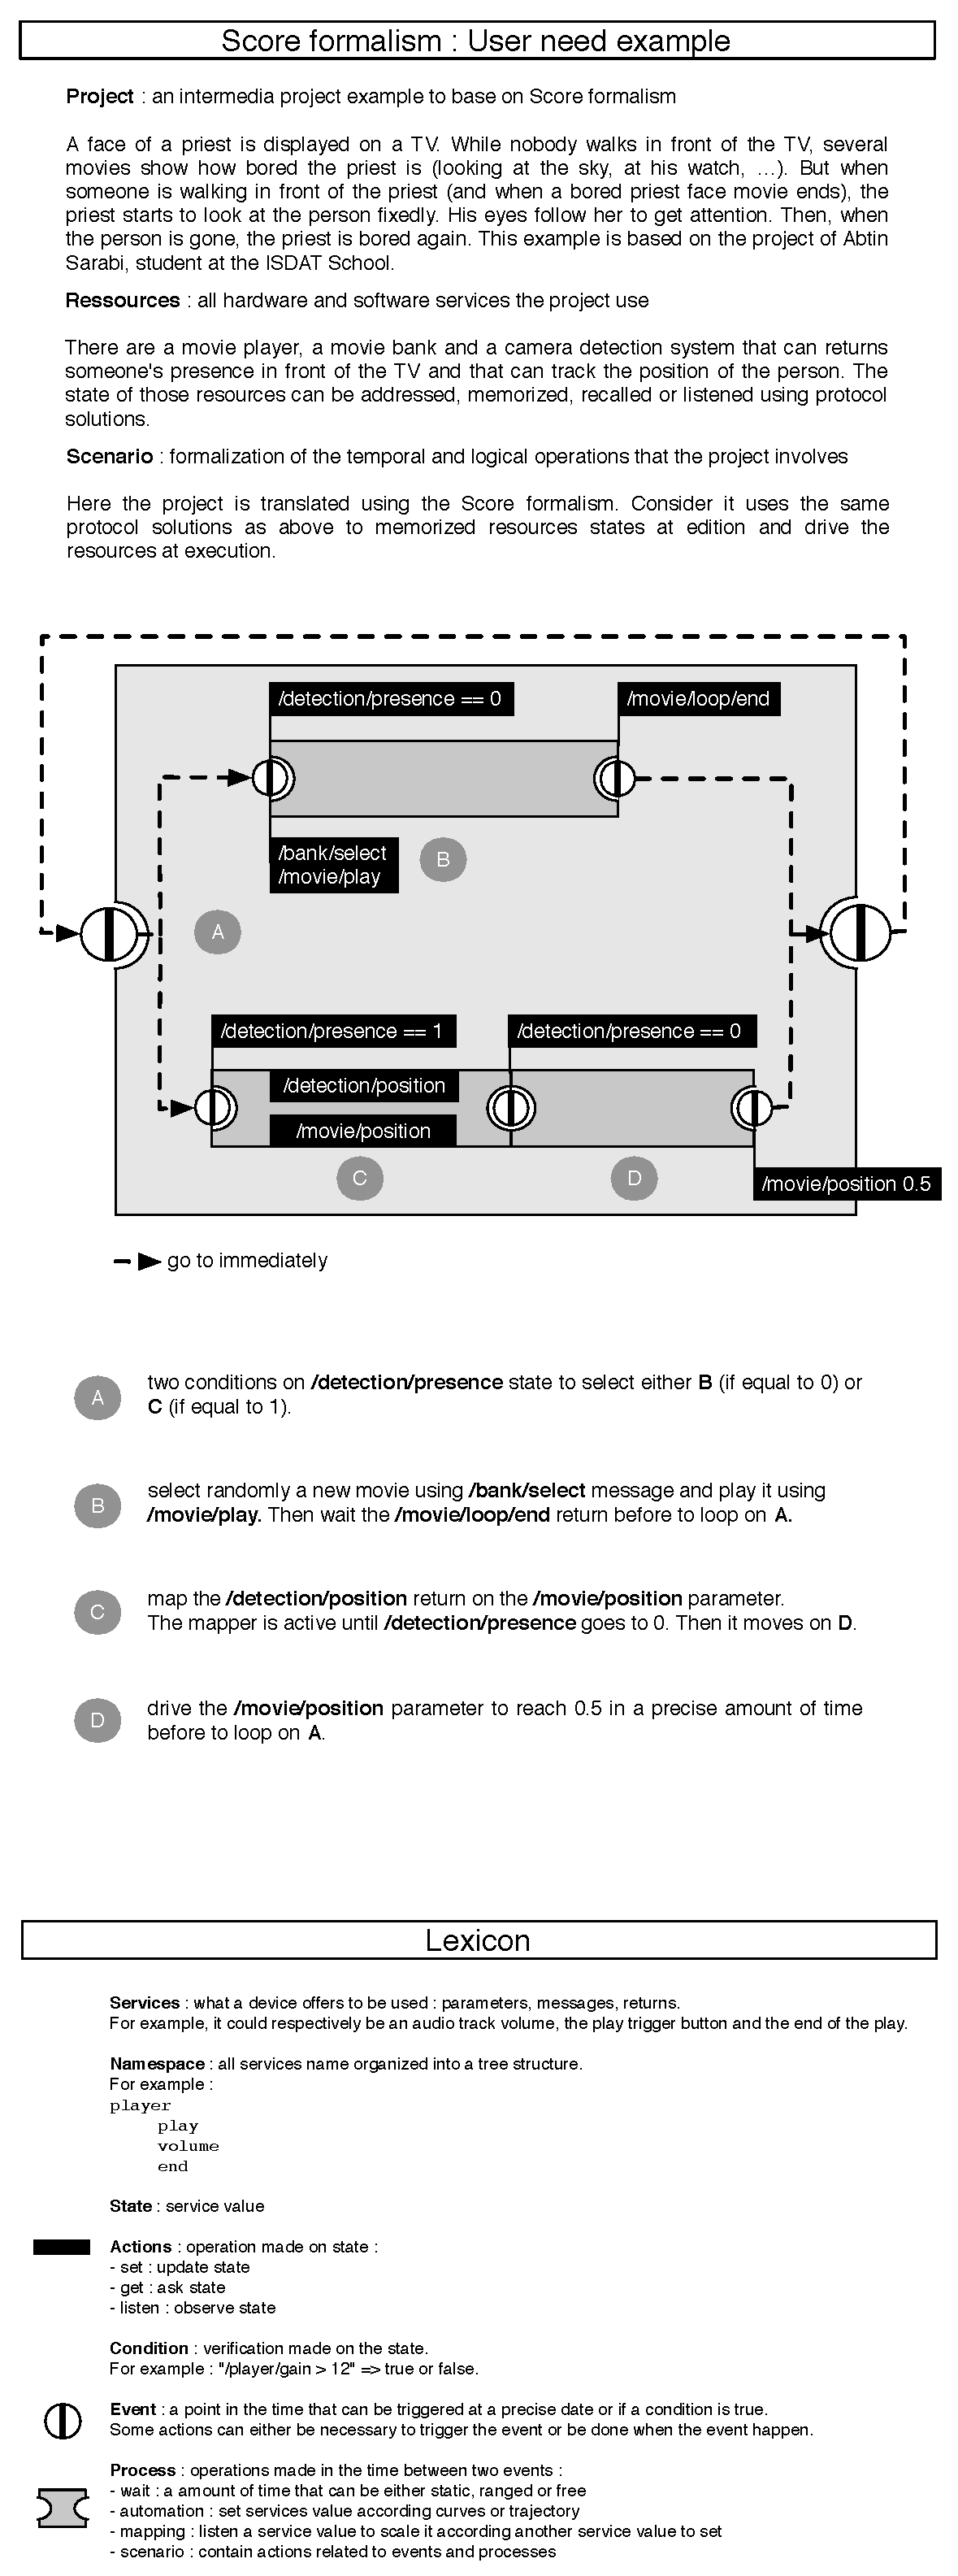
\includegraphics[clip,trim=0cm 28cm 0cm 0cm, width=1.00\textwidth]{images/moineOSSIA.pdf}
	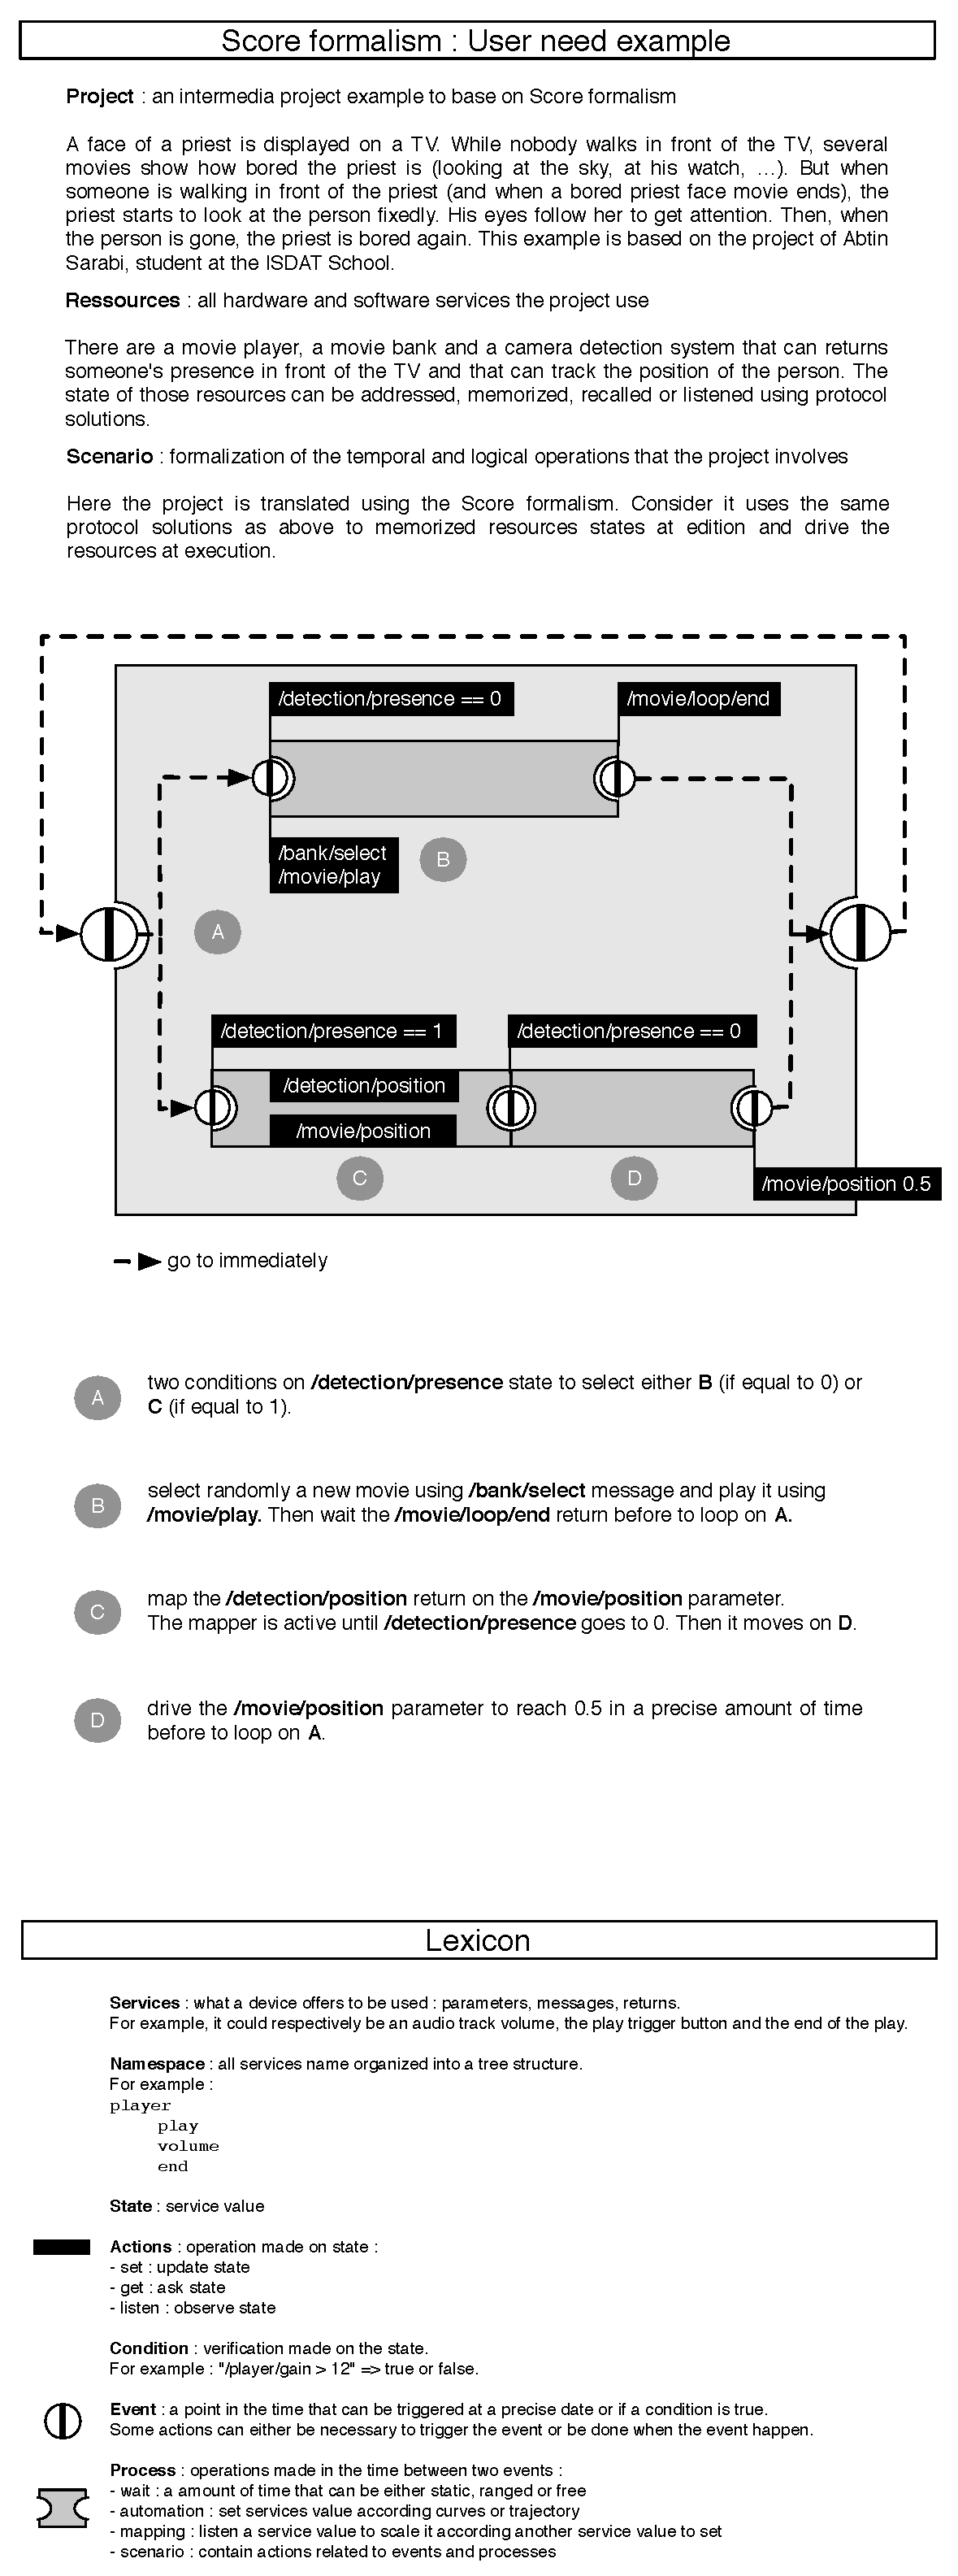
\includegraphics[clip,trim=0cm 0cm 0cm 26cm, width=1.00\textwidth]{images/moineOSSIA.pdf}
	
	\chapter{Captures d'écran : exemples d'exécution sur machines virtuelles}
	\begin{figure}
		\centering
		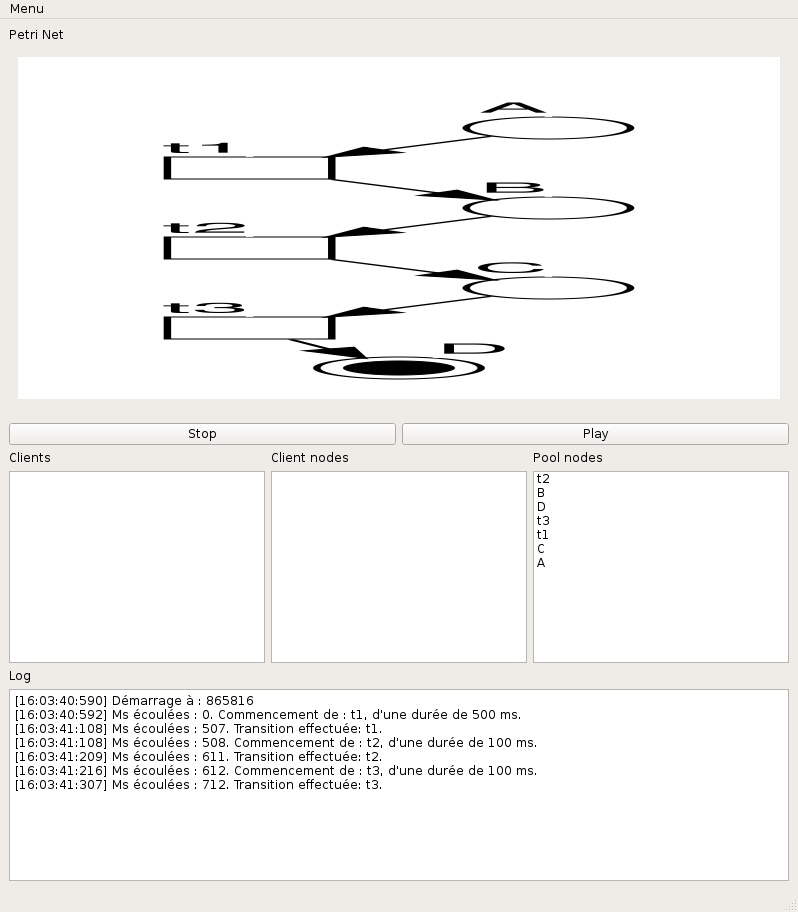
\includegraphics[scale=0.55]{images/resultats/vm/serverVMideal.png}
		
		\caption{Exécution idéale sur une machine virtuelle}
		\label{fig.executionTheoriqueVM}
	\end{figure}

	\begin{sidewaysfigure}
		\centering
		\begin{tabular}{rl}
			\begin{subfigure}{0.5\textwidth}
				\centering
				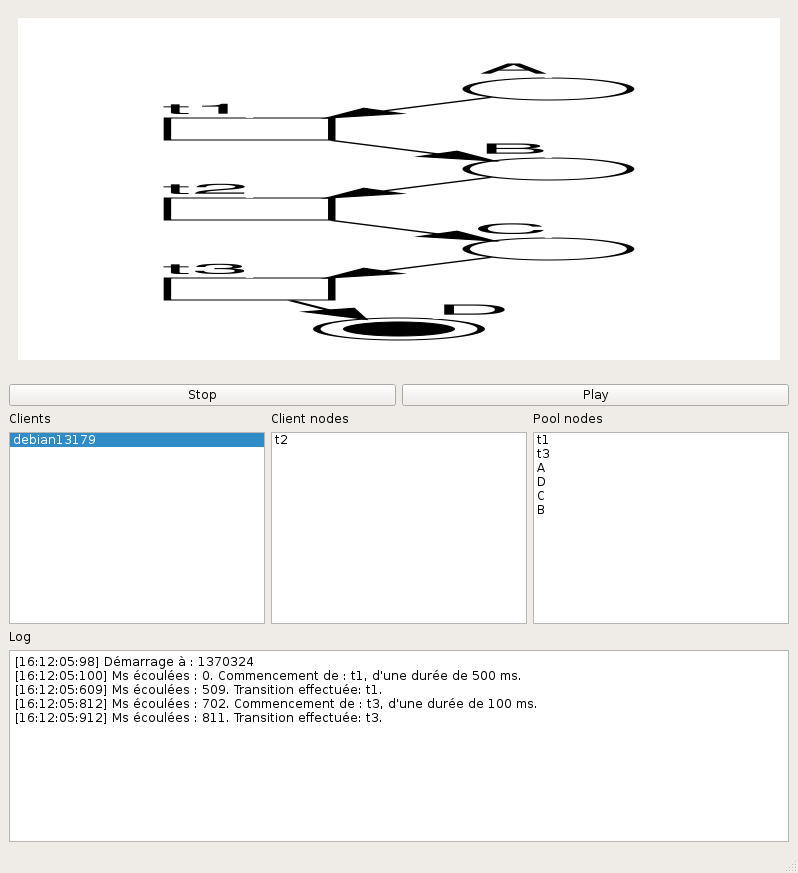
\includegraphics[scale=0.45]{images/resultats/vm/serverVMsimple.png}
				\caption{Serveur}
			\end{subfigure}
			&
			\begin{subfigure}{0.5\textwidth}
				\centering
				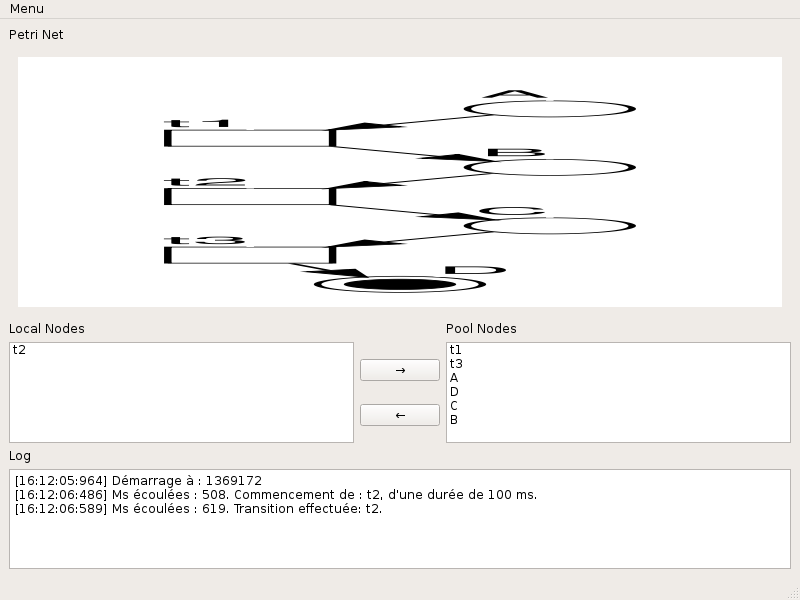
\includegraphics[scale=0.45]{images/resultats/vm/clientVMsimple.png}
				\caption{Client}
			\end{subfigure}
		\end{tabular}
		
		\caption{Exécution naïve sur machines virtuelles}
		\label{fig.simpleVM}
	\end{sidewaysfigure}
	
	\begin{sidewaysfigure}
		\centering
		\begin{tabular}{rl}
			\begin{subfigure}{0.5\textwidth}
				\centering
				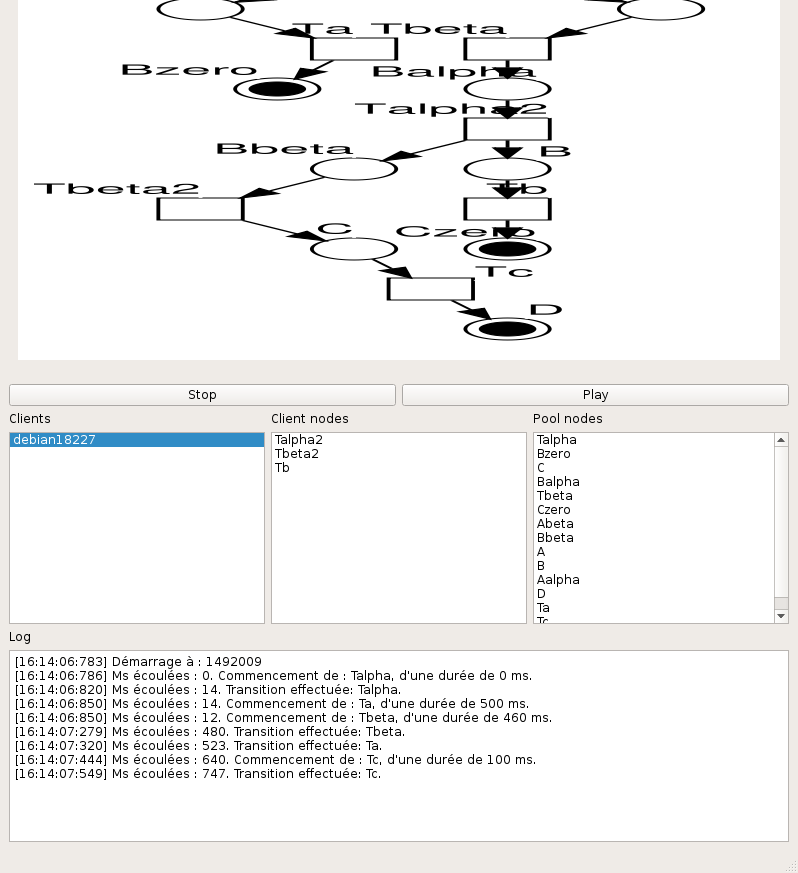
\includegraphics[scale=0.45]{images/resultats/vm/serverVMalgo.png}
				\caption{Serveur}
			\end{subfigure}
			&
			\begin{subfigure}{0.5\textwidth}
				\centering
				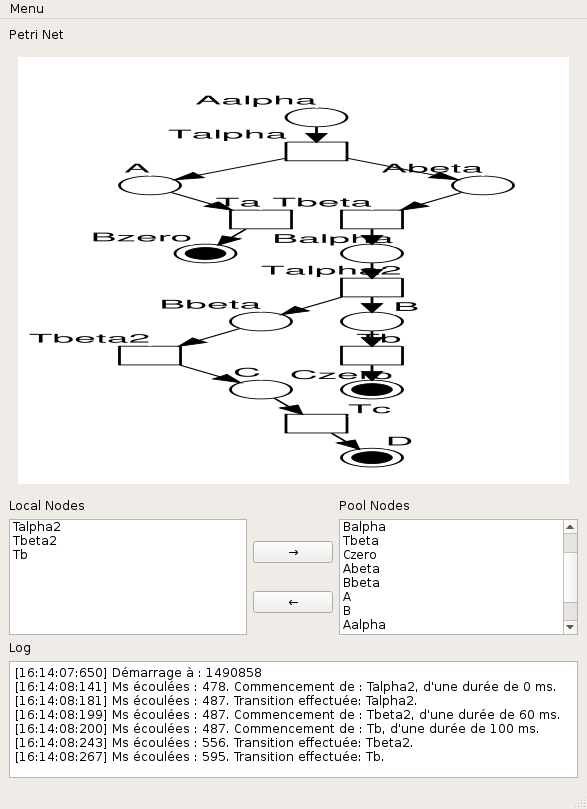
\includegraphics[scale=0.45]{images/resultats/vm/clientVMalgo.png}
				\caption{Client}
			\end{subfigure}
		\end{tabular}
		
		\caption{Exécution avec algorithme sur machines virtuelles}
		\label{fig.algoVM}
	\end{sidewaysfigure}
	
	\chapter{Captures d'écran : exemples d'exécution avec tablette}
	\begin{figure}
		\centering
		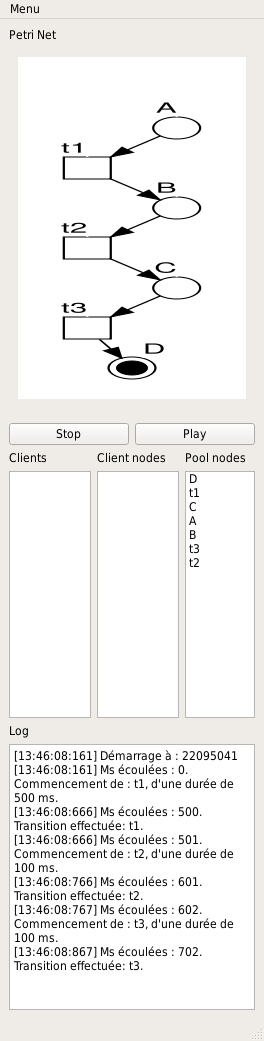
\includegraphics[scale=0.45]{images/resultats/server_simple_correct.png}
		
		\caption{Exécution idéale sur ordinateur}
		\label{fig.executionTheorique}
	\end{figure}
	
	\begin{sidewaysfigure}
		\centering
		\begin{tabular}{rl}
		\begin{subfigure}{0.5\textwidth}
			\centering
			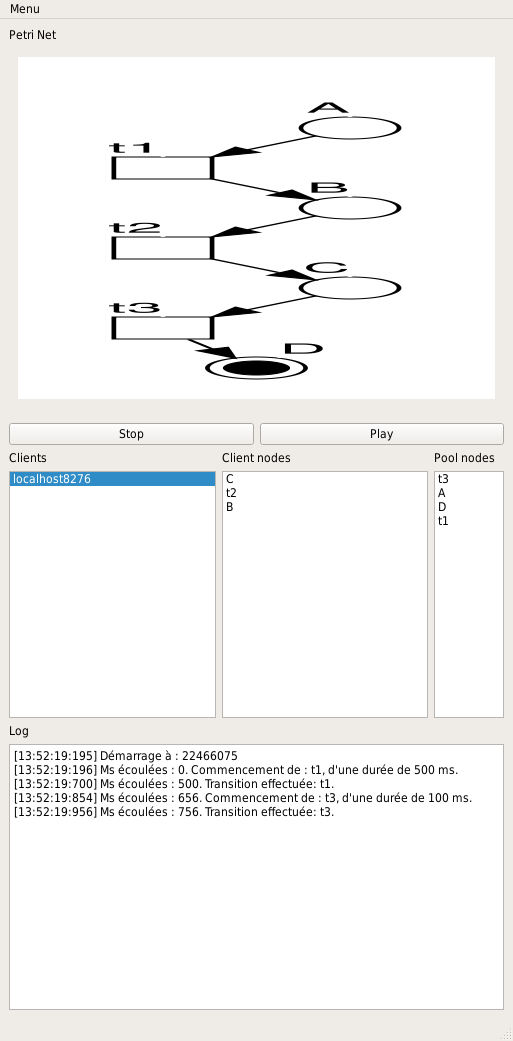
\includegraphics[scale=0.45]{images/resultats/server_simple_wifi.png}
			\caption{Serveur}
		\end{subfigure}
		 &
		\begin{subfigure}{0.5\textwidth}
			\centering
			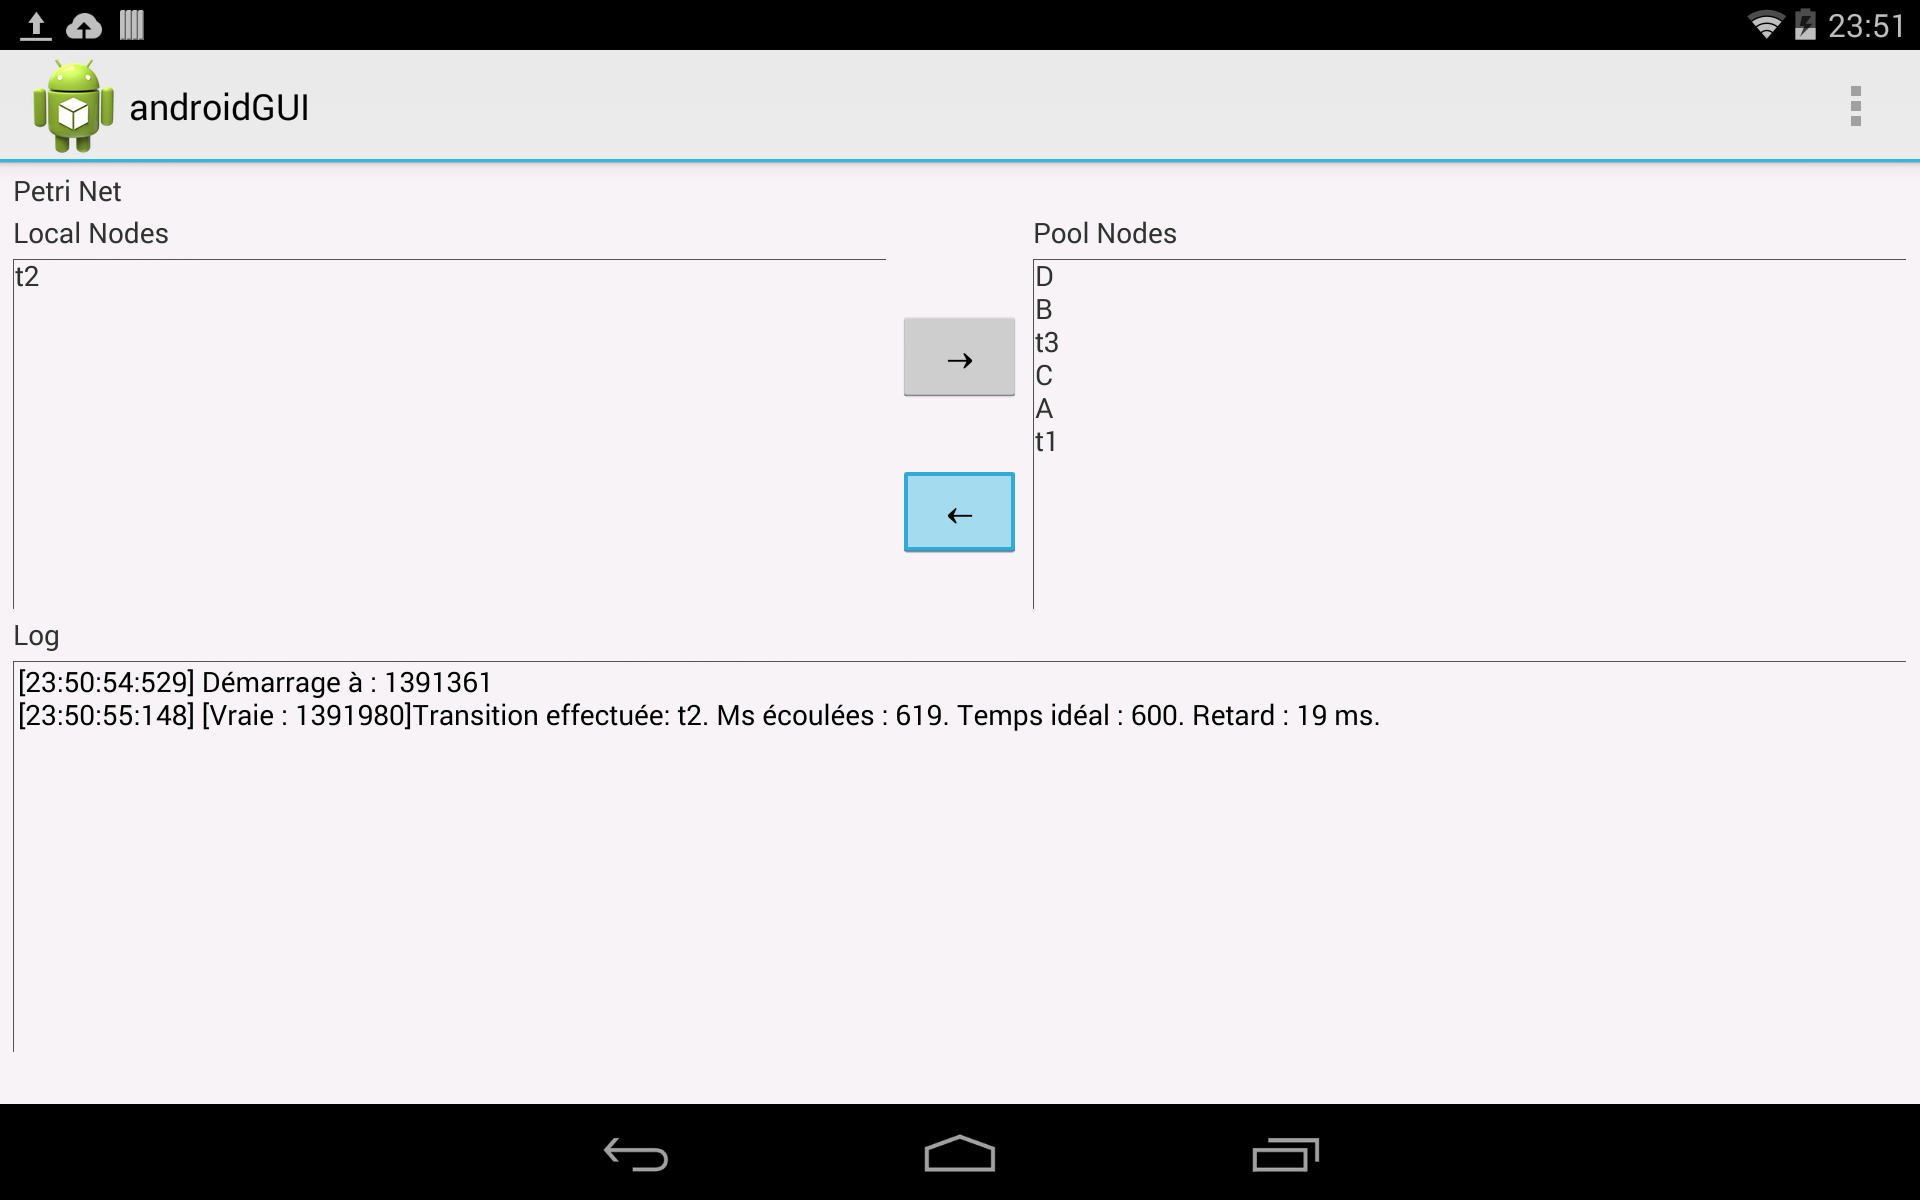
\includegraphics[scale=0.22]{images/resultats/client_simple_wifi.png}
			\caption{Client}
		\end{subfigure}
		\end{tabular}
		
		\caption{Exécution naïve sur tablette}
		\label{fig.androSimpl}
	\end{sidewaysfigure}
	
	
	\begin{sidewaysfigure}
		\centering
		\begin{tabular}{rl}
		\begin{subfigure}{0.5\textwidth}
			\centering
			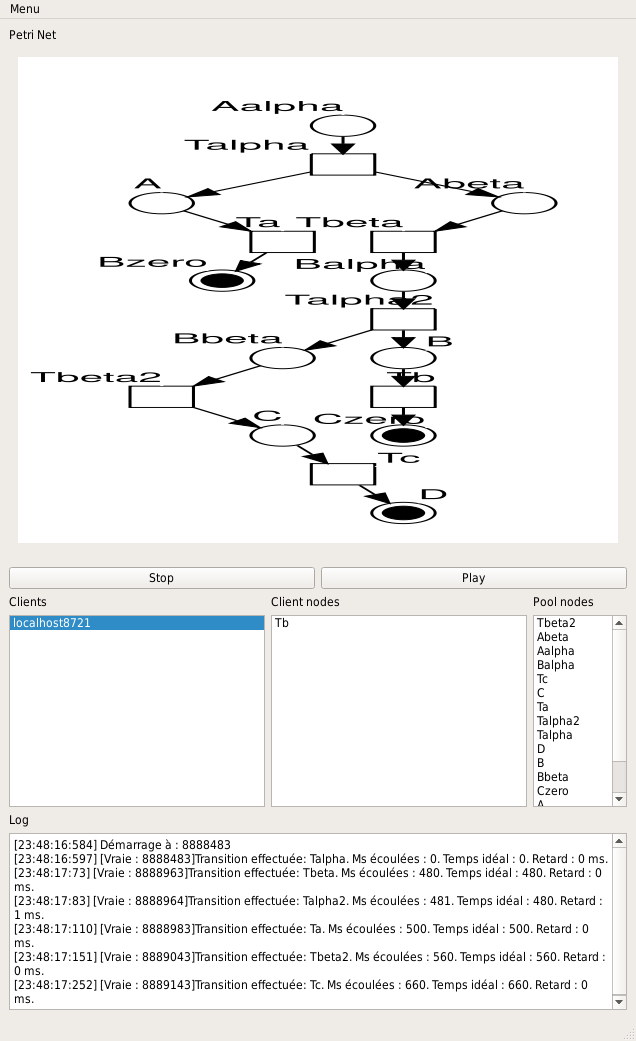
\includegraphics[scale=0.45]{images/resultats/server_algo_wifi.png}
			\caption{Serveur}
		\end{subfigure}
		&
		\begin{subfigure}{0.5\textwidth}
			\centering
			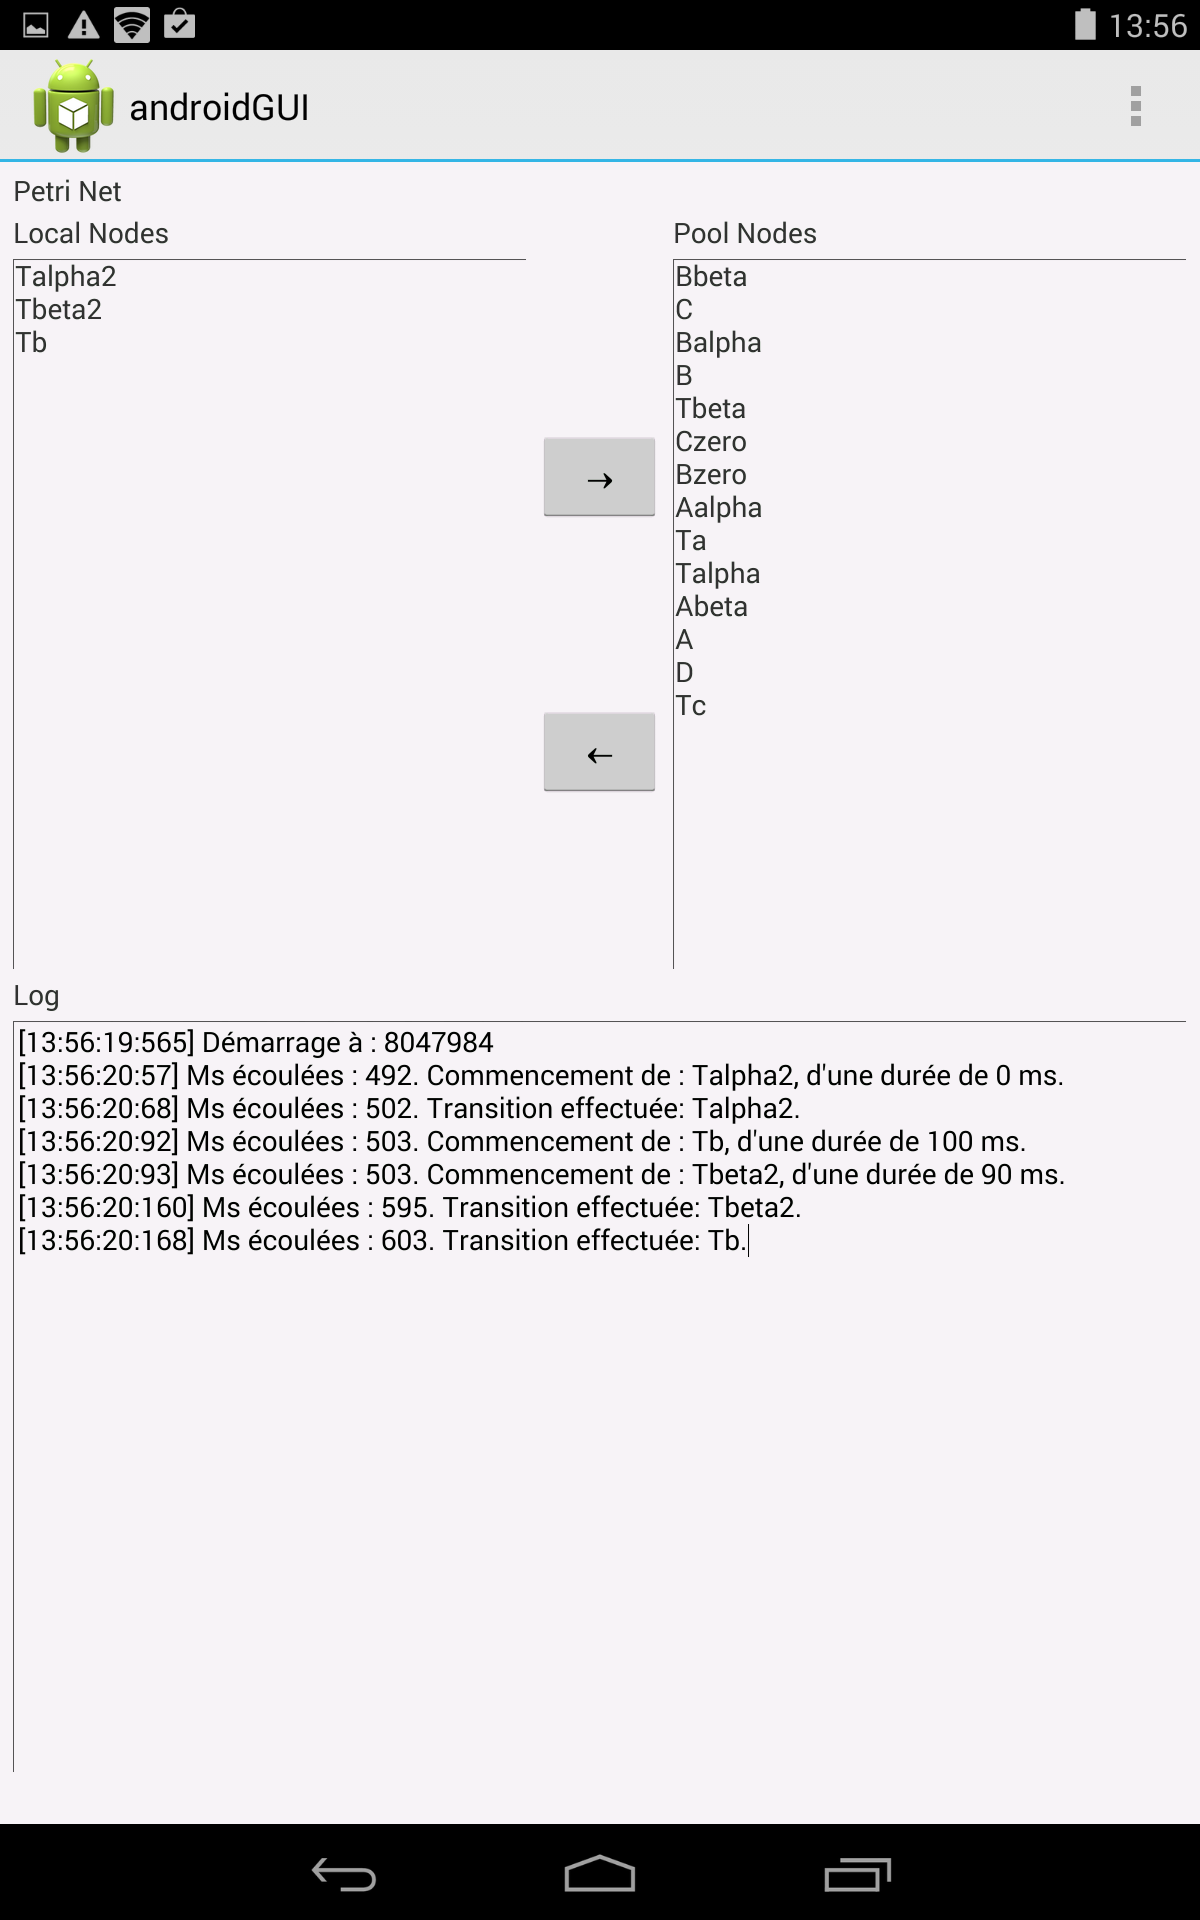
\includegraphics[scale=0.22]{images/resultats/client_algo_wifi.png}
			\caption{Client}
		\end{subfigure}
		\end{tabular}
		
		\caption{Exécution avec algorithme de déplacement sur tablette}
		\label{fig.androDepl}
	\end{sidewaysfigure}
	
	
\printglossaries
\bibliographystyle{alpha}
\bibliography{stagepetri}
\end{document}
